
%%%%
%%%%  FIGURE 
%%%%
\begin{figure}[h]
\vbox{\vspace{0.cm}
\hbox{\hspace{2cm}
\includegraphics[width=.5\textwidth]{./Pics/P1DGP2.pdf}}
\vspace{0.cm}
\hbox{\hspace{5cm}(a)}
\vspace{0.5cm}
\hbox{\hspace{1cm}
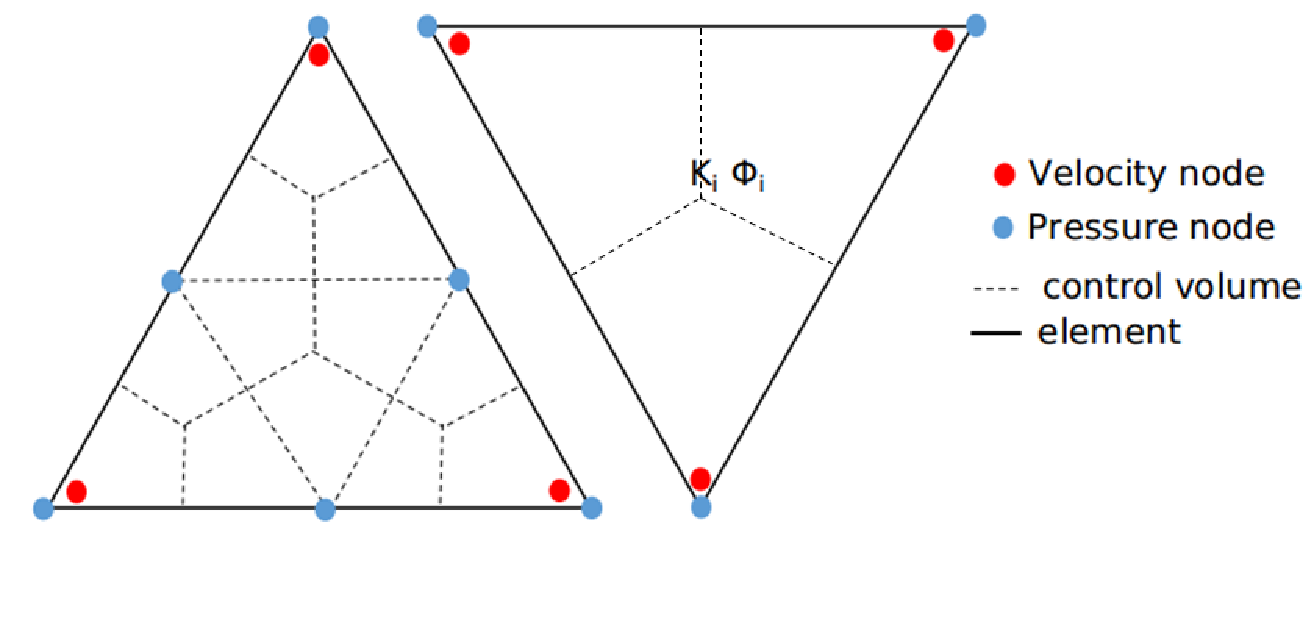
\includegraphics[width=.75\textwidth]{./Pics/element_n_2b.pdf}}
\vspace{0.cm}
\hbox{\hspace{3.5cm}(b)\hspace{3cm}(c)}}
%\vbox{\includegraphics[width=.5\textwidth]{./Pics/P1DGP2.pdf}}
\caption{2D representation of \PN[n]{m} element-pairs used in this work: (a) set of \PN[1]{2} FE with shaded areas as control volumes across two contiguous elements (blue and white circles represent pressure and velocity nodes, respectively). Detailed (b) \PN[1]{2} and (c) \PN[1]{1} element-pairs.} 
\label{fig:fem_elem}
\end{figure}
\clearpage


%%%%
%%%%  FIGURE
%%%%
%\begin{figure}[h]
%\centering
%\vbox{\includegraphics[width=.75\textwidth]{./Pics/element_n_1.pdf}}
%\vbox{\includegraphics[width=.75\textwidth]{./Pics/element_n_2.pdf}}
%\caption{Graphical representation of two different element-types: triangles {\it A} and {\it B} represent \PN[1]{2} and \PN[1]{1} element-pairs, respectively. Porosity $\phi_{i}$, permeability {\bf K}$_{i}$, velocity and pressure are represented in FE space whereas scalar fields (such as saturation, density, viscosity etc) are represented in CV space.}
%\label{fig:fem_elem}
%\end{figure}
%\clearpage

%%%%
%%%%  FIGURE 
%%%%
%\begin{figure}[h]
%\centering
%\vbox{\includegraphics[width=0.75\textwidth]{./Pics/phase_vol_frac_uni_perm_1.pdf}}
%\vbox{\includegraphics[width=0.75\textwidth]{./Pics/phase_vol_frac_uni_perm_2.pdf}}
%\caption{Schematics of formation of flow instabilities during injection of a pure low viscosity fluid (red) into a domain saturated with a second fluid (dark blue). The viscocity ratio of the two fluids is VR=$5$. In this case, the initially piston shape front collapses leading to the formation of several fingers.}
%\label{fig:simple_case}
%\end{figure}
%\clearpage


%%%%
%%%%  FIGURE 
%%%%
%\begin{figure}[ht] 
%\vbox{
%\hbox{\hspace{-0.3cm}
%\includegraphics[width=.8\textwidth]{./Pics1/2b2_wi_fine/2b2_whole_in_fine_perm_1.pdf} 
%\includegraphics[width=.8\textwidth]{./Pics1/2b2_wi_fine/2b2_whole_in_fine_perm_2.pdf} 
%}
%\vspace{0.0cm}
%\hbox{\hspace{3.5cm} (a) Schematics of the domain with permeability ($\mathbf{K}$) distribution
%}
%\vspace{0.25cm}
%\hbox{\hspace{1.5cm}
%\includegraphics[width=.85\textwidth]{./Pics1/2b2_wi_fine/2b2_whole_in_fine_250_2.pdf}
%}
%\vspace{0.0cm}
%\hbox{\hspace{4.5cm} (b) flow at t=25
%}
%\vspace{0.25cm}
%\hbox{\hspace{1.5cm}
%\includegraphics[width=.65\textwidth]{./Pics1/2b2_wi_fine/2b2_whole_in_fine_3000_2.pdf}
%}
%\vspace{0.0cm}
%\hbox{\hspace{4.0cm} (c) flow at t=3000   
%}}     
%\caption{Model validation of fluid displacement in heterogeneous porous media ({\it VR}=1): (a) the domain is divided into four subdomains with prescribed synthetic permeability, $\mathbf{K}_{1}=2.5$ and $\mathbf{K}_{2}=1$; (b-c) snapshots of saturation (displacing fluid) field at t=$25$ and t=$300$. The domain is discretised with $5960$ \PN[1]{2} elements. }
%\label{DaweGrattoniExperiment_a}
%\end{figure}
%\clearpage
%\end{comments}


%%%%
%%%%  FIGURE
%%%%
\begin{figure}[ht] 
    \vbox{
       \hbox{\hspace{1.cm}\includegraphics[width=\textwidth]{./Pics1/2b2_wi_fine/2b2_whole_in_fine_perm_2}}
       \vspace{0.cm}
       \hbox{\hspace{7cm}(a)}
       \vspace{0.cm}
       \hbox{\hspace{1.cm}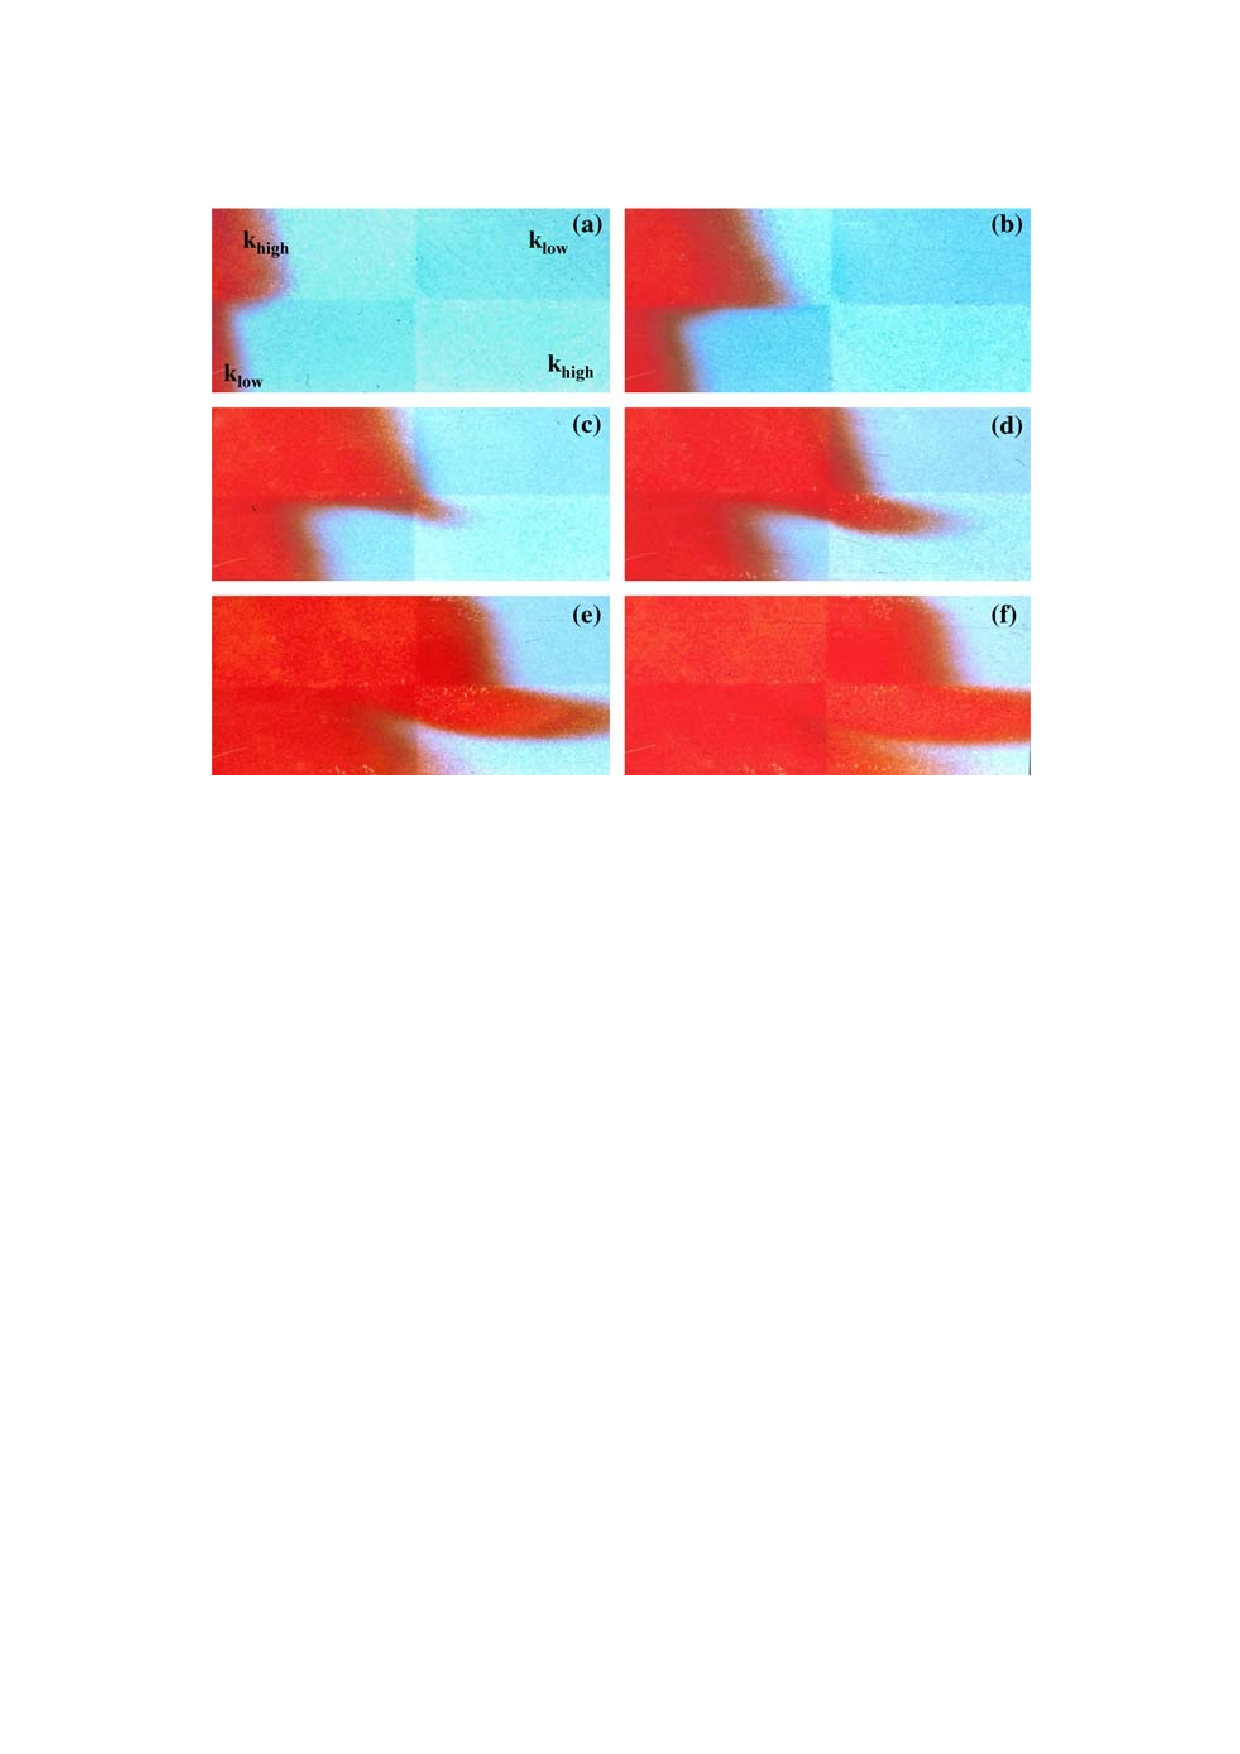
\includegraphics[width=\textwidth]{./Pics1/DaweGrattoni_Experiment/1pageb}}
       \vspace{0.cm}
       \hbox{\hspace{7cm}(b)}
    }   
\caption{Model validation of fluid displacement in heterogeneous porous media ({\it VR}=1): (a) sketch of the the domain which is divided into four subdomains with prescribed synthetic permeability, $\mathbf{K}_{1}=2.5$ and $\mathbf{K}_{2}=1$; (b) fluid displacement with permeability ratio of 2.5, exttracted from \citet{dawe_2008}. }
\label{DaweGrattoniExperiment_a}
\end{figure}
\clearpage




%%%%
%%%%  FIGURE
%%%%
\begin{landscape}
  \begin{figure}[ht] 
    \vbox{\vspace{0.cm}
       \hbox{\hspace{1cm}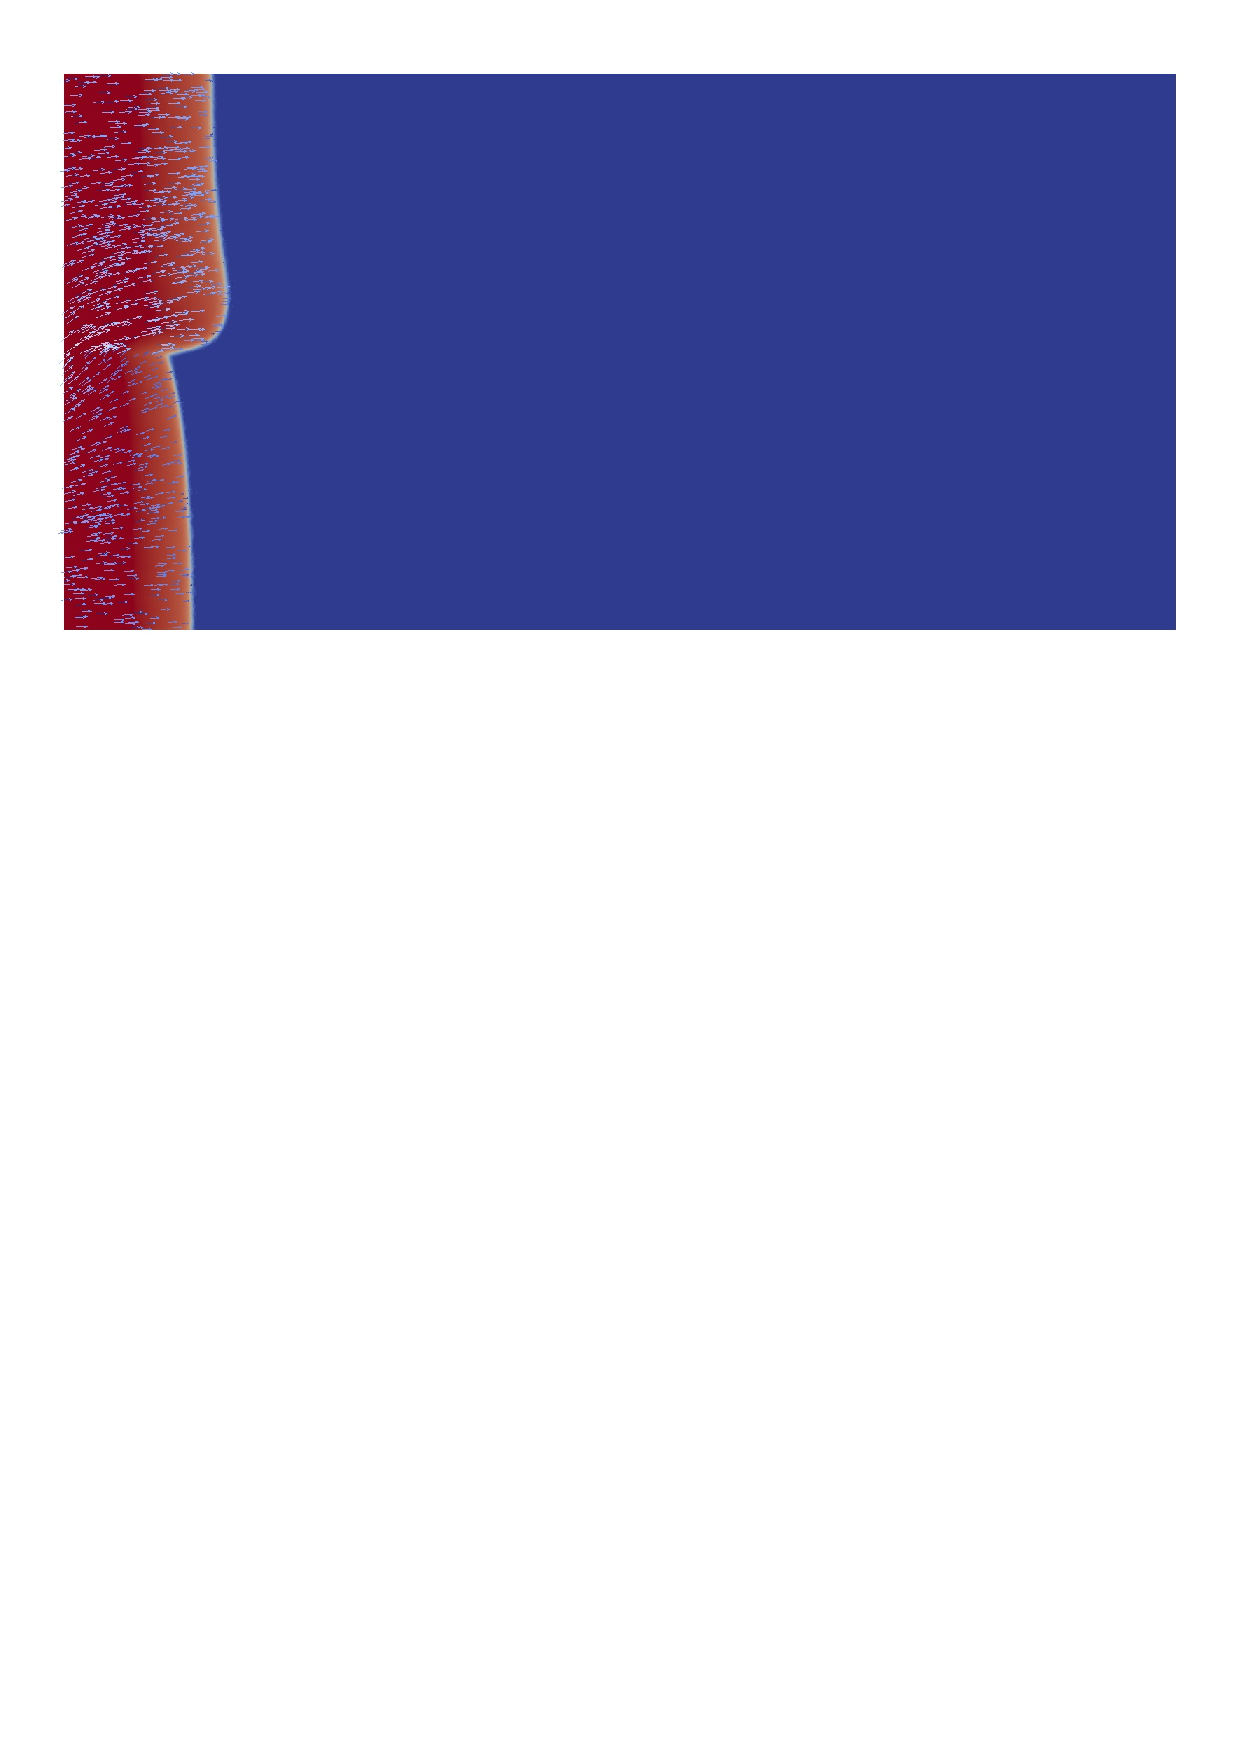
\includegraphics[width=.50\textwidth]{./Pics1/DaweGrattoni_Experiment/CrossFlow_d61b}  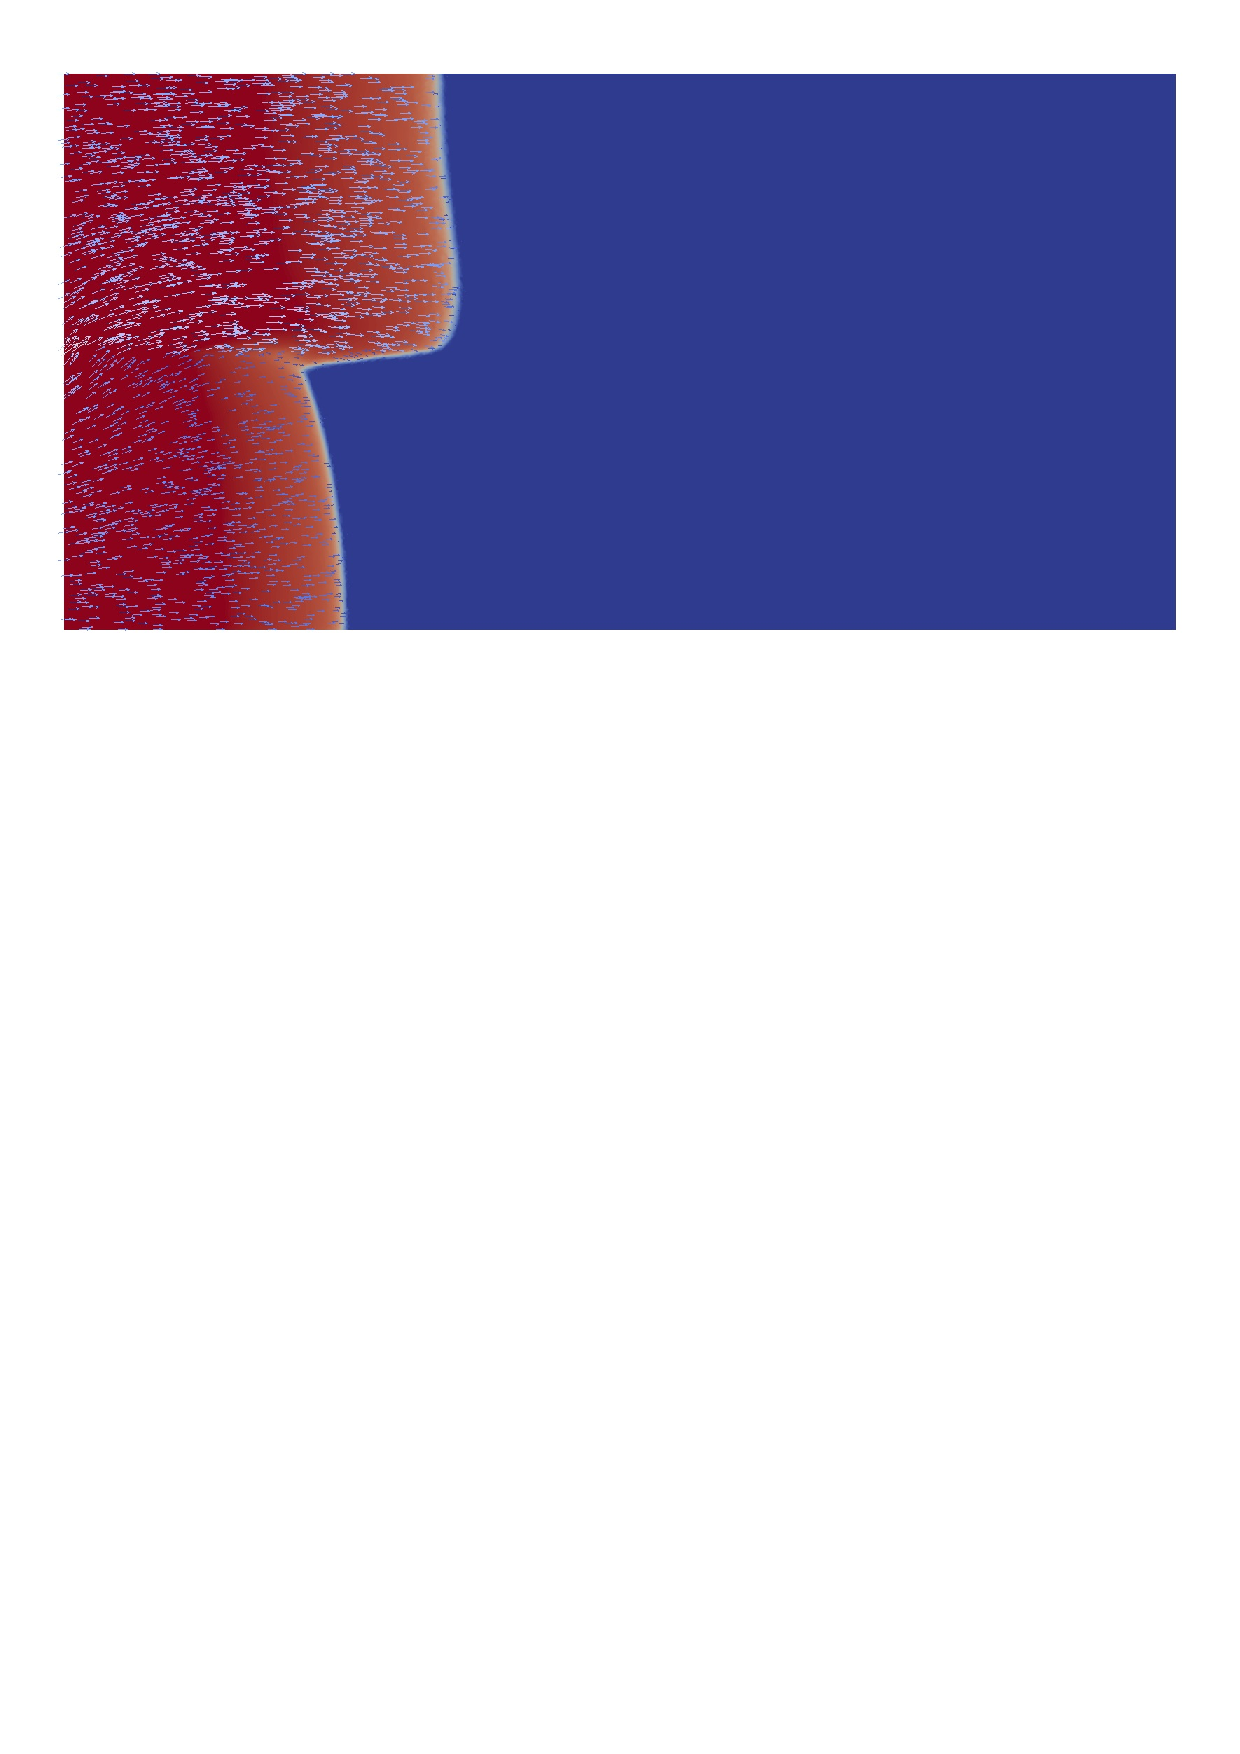
\includegraphics[width=.50\textwidth]{./Pics1/DaweGrattoni_Experiment/CrossFlow_d125b}  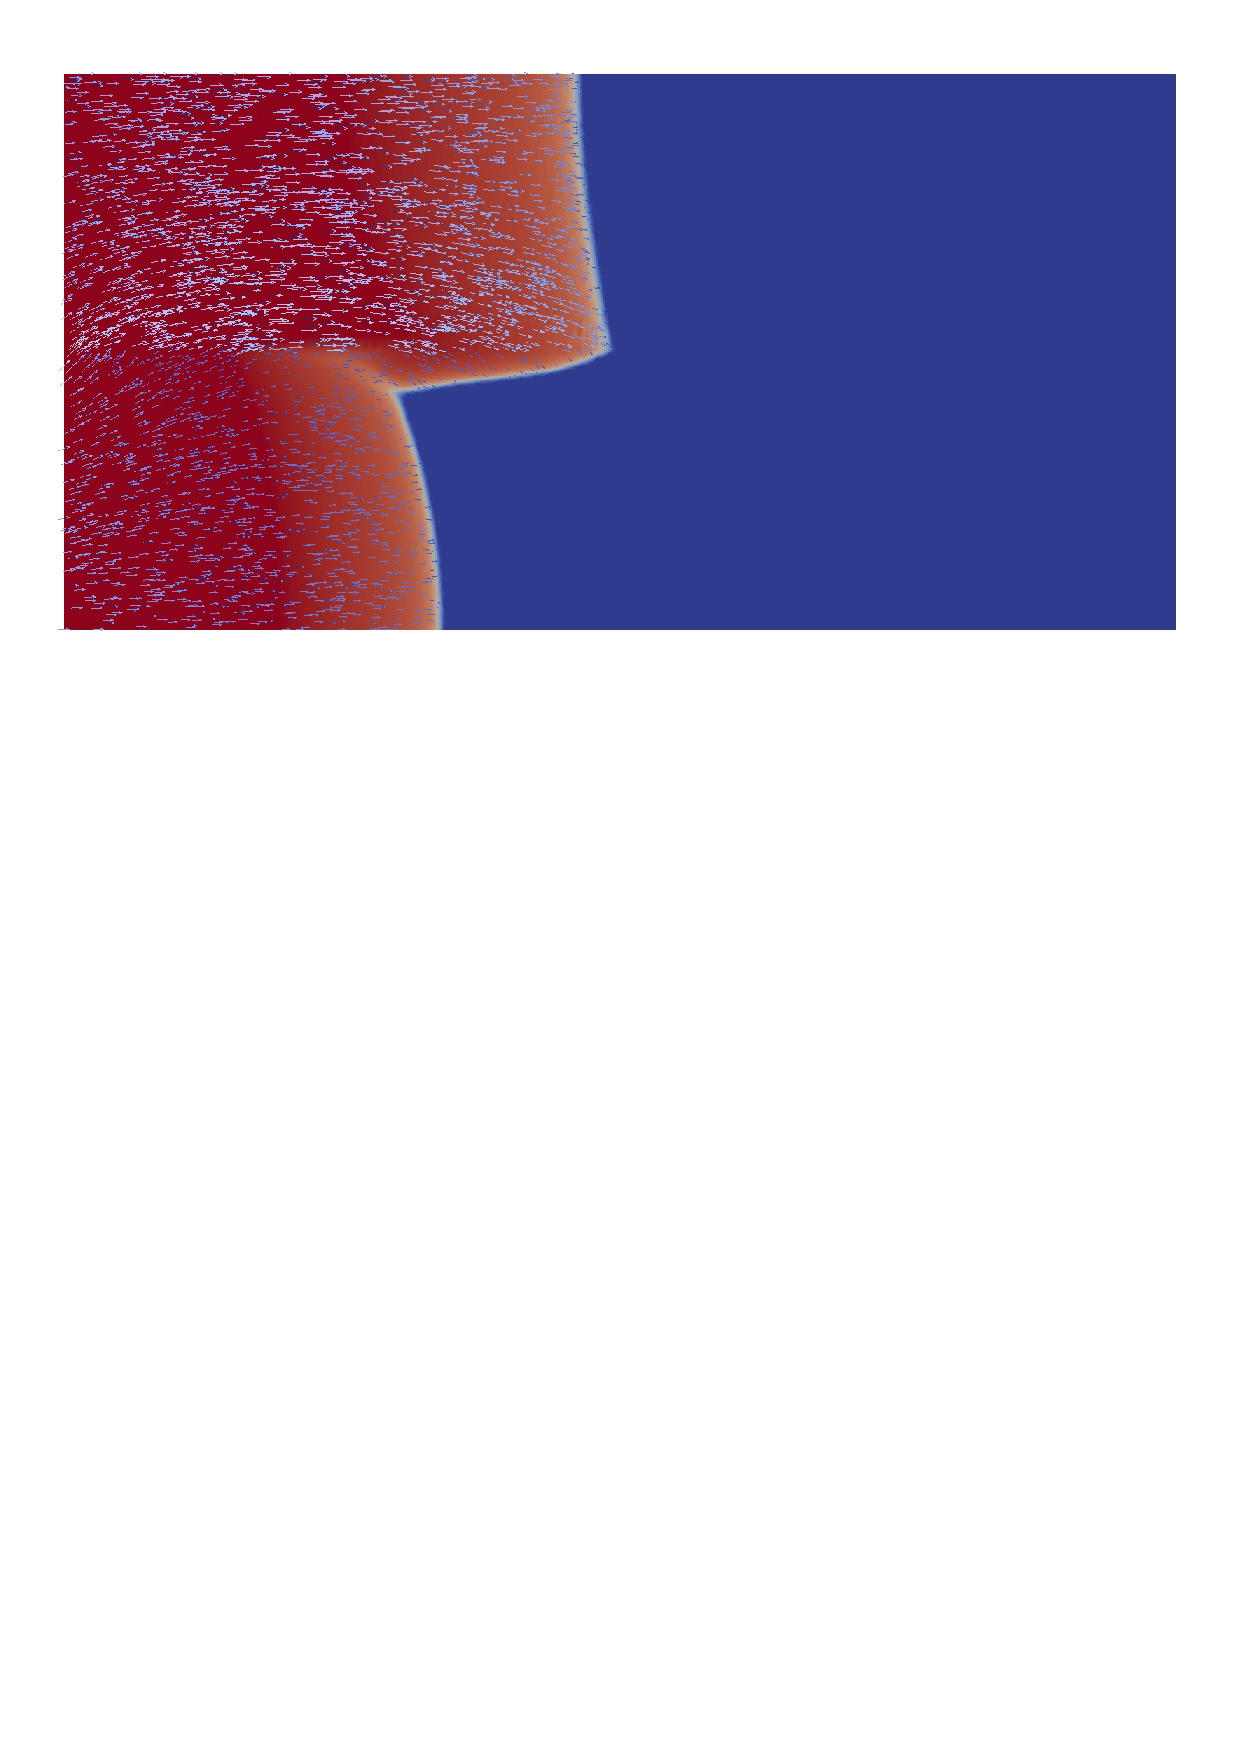
\includegraphics[width=.50\textwidth]{./Pics1/DaweGrattoni_Experiment/CrossFlow_d145b} }
       \hbox{\hspace{1cm}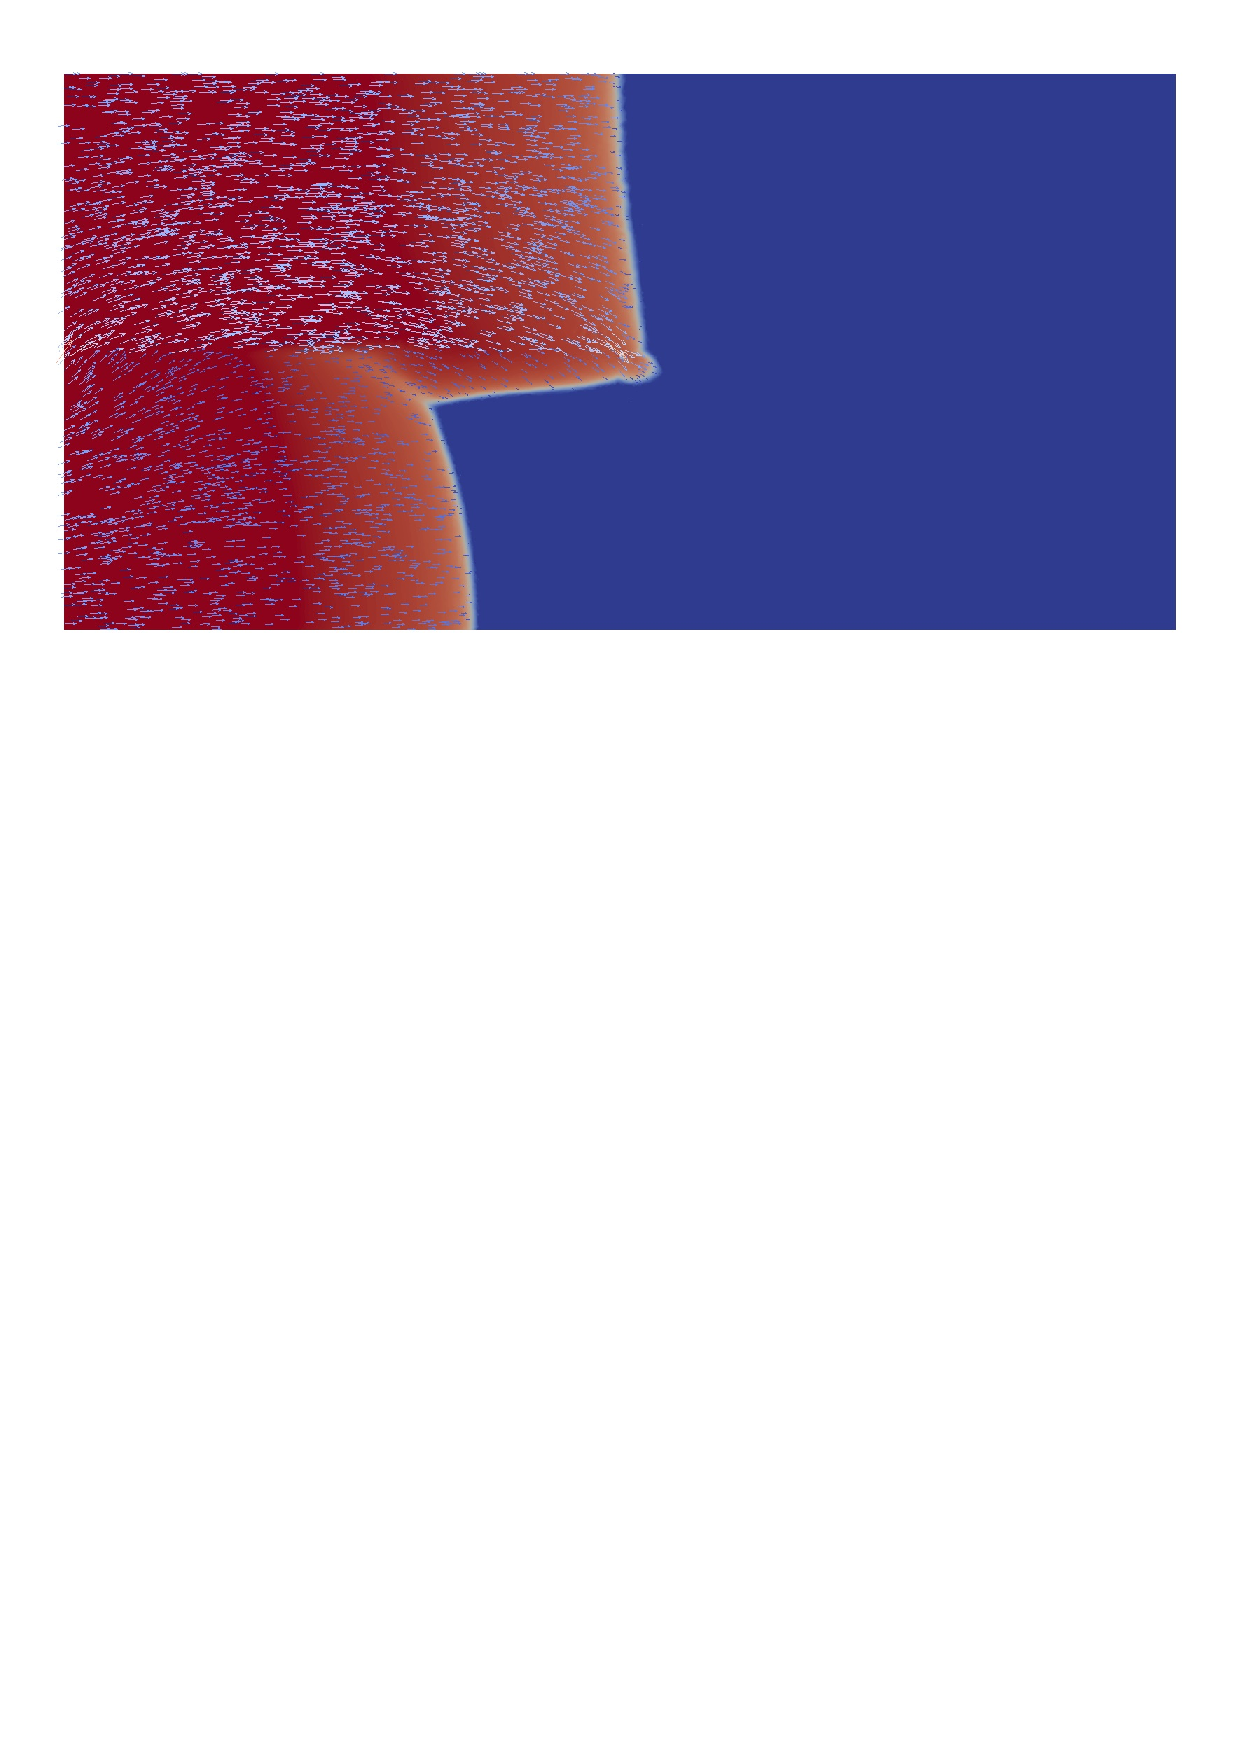
\includegraphics[width=.50\textwidth]{./Pics1/DaweGrattoni_Experiment/CrossFlow_d152b}  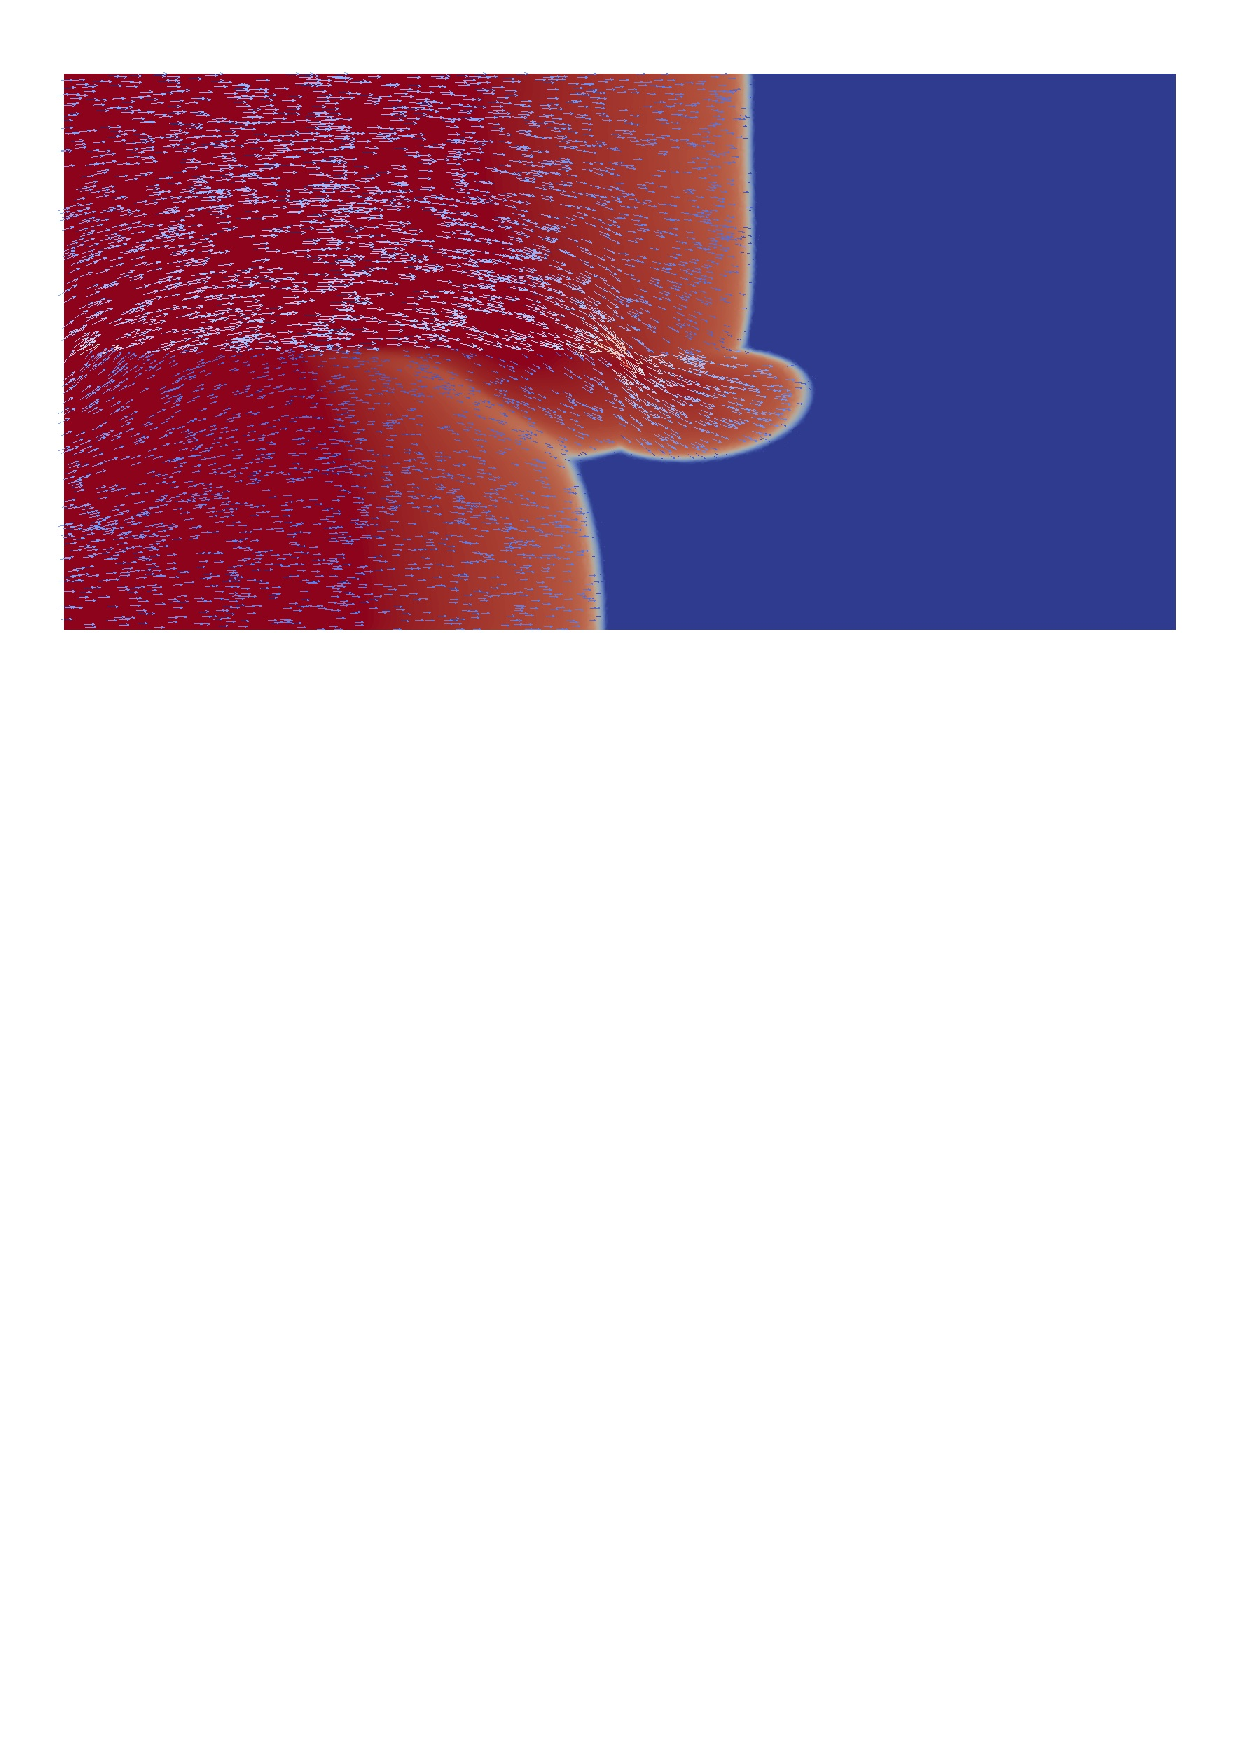
\includegraphics[width=.50\textwidth]{./Pics1/DaweGrattoni_Experiment/CrossFlow_d180b}  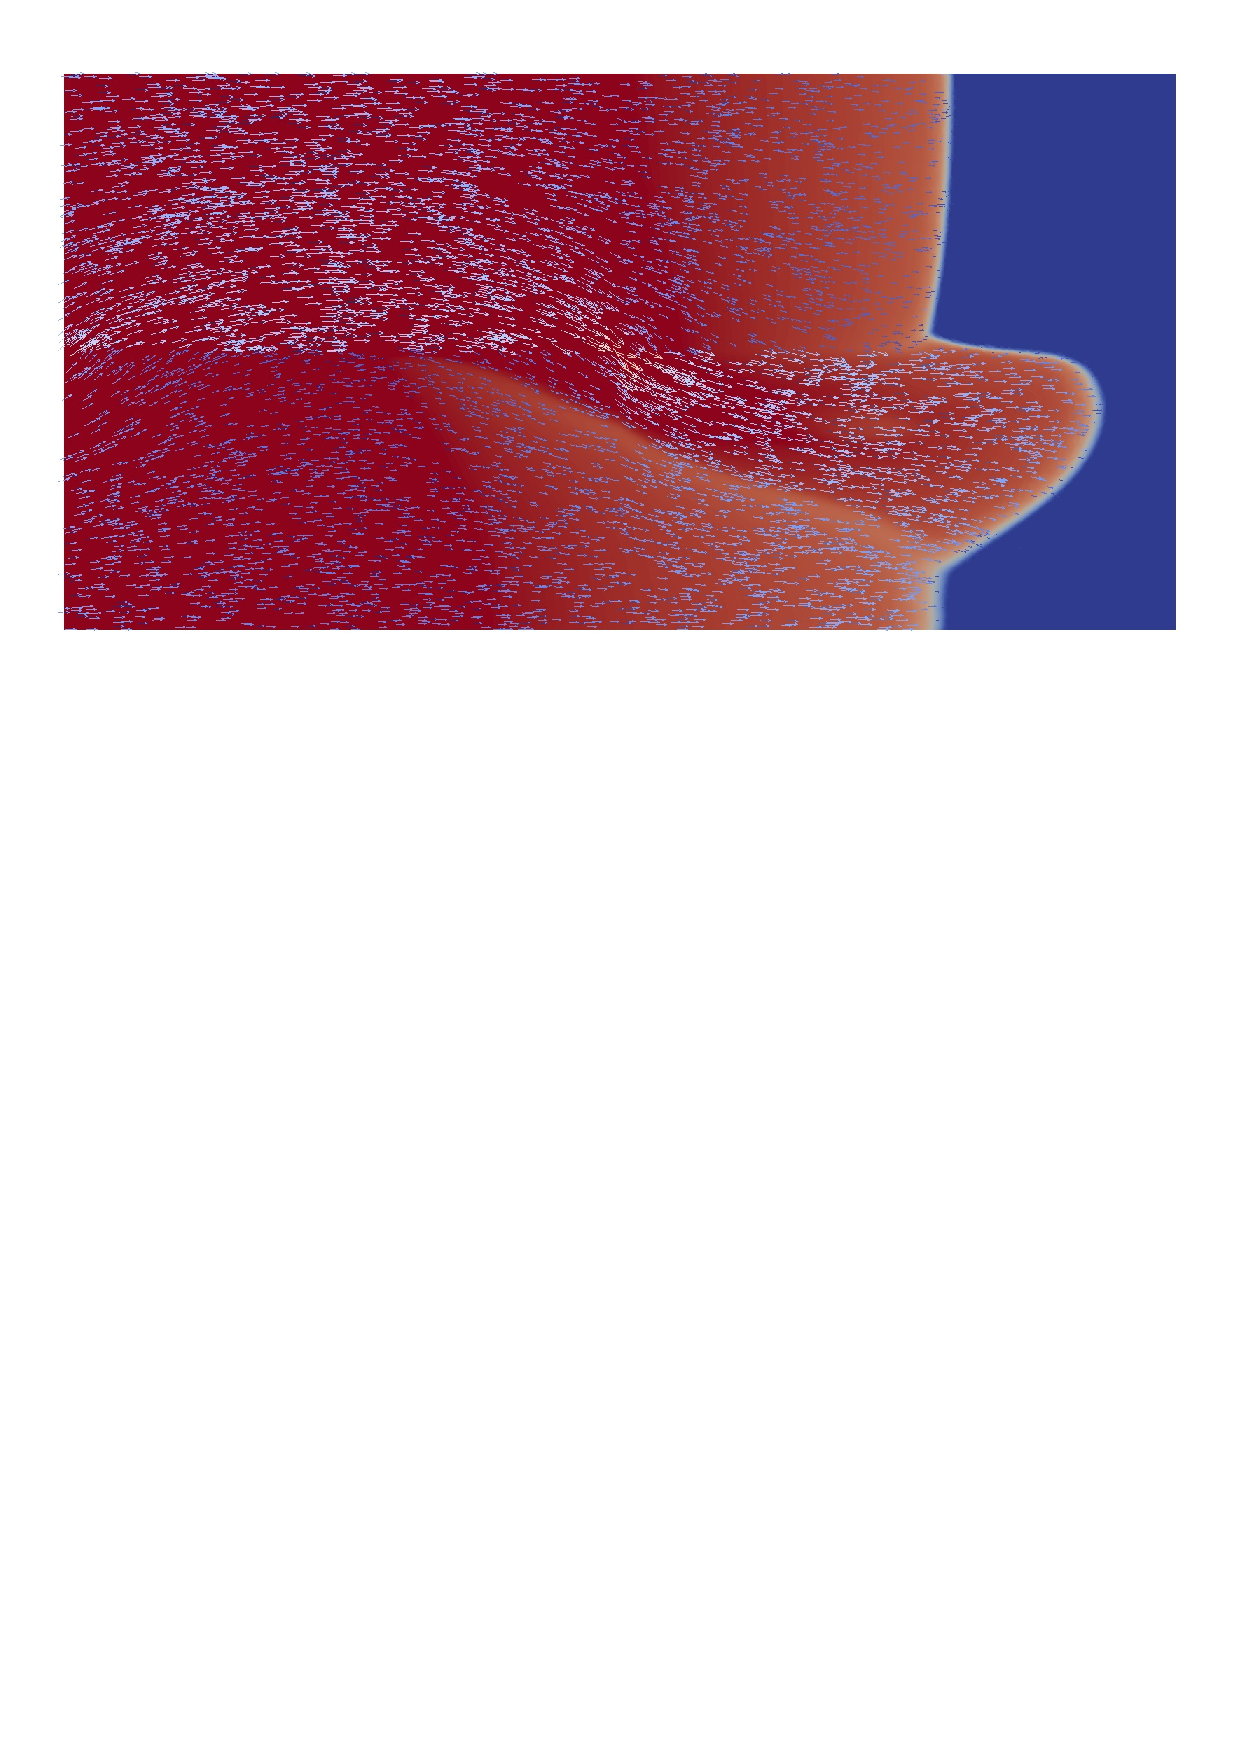
\includegraphics[width=.50\textwidth]{./Pics1/DaweGrattoni_Experiment/CrossFlow_d250b} }
       \hbox{\hspace{1cm}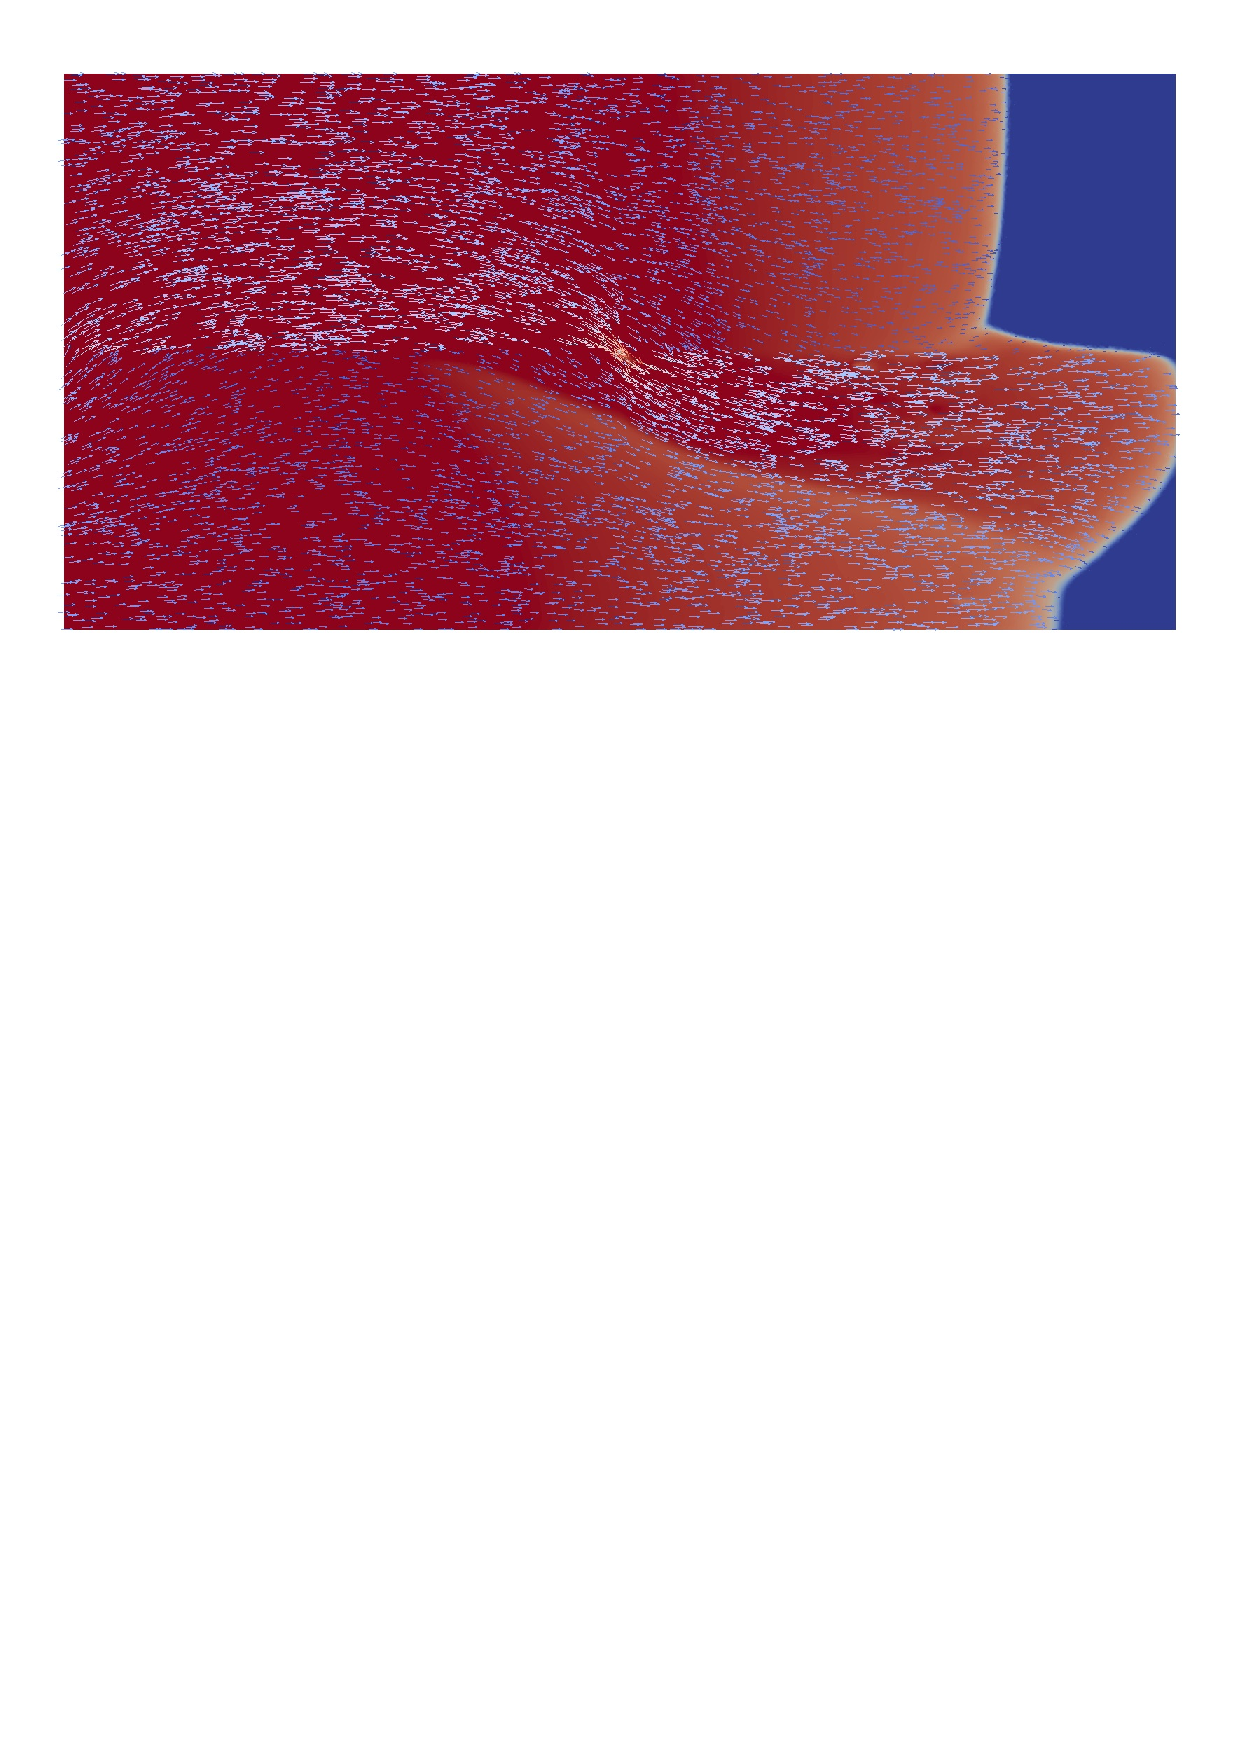
\includegraphics[width=.50\textwidth]{./Pics1/DaweGrattoni_Experiment/CrossFlow_d260b}  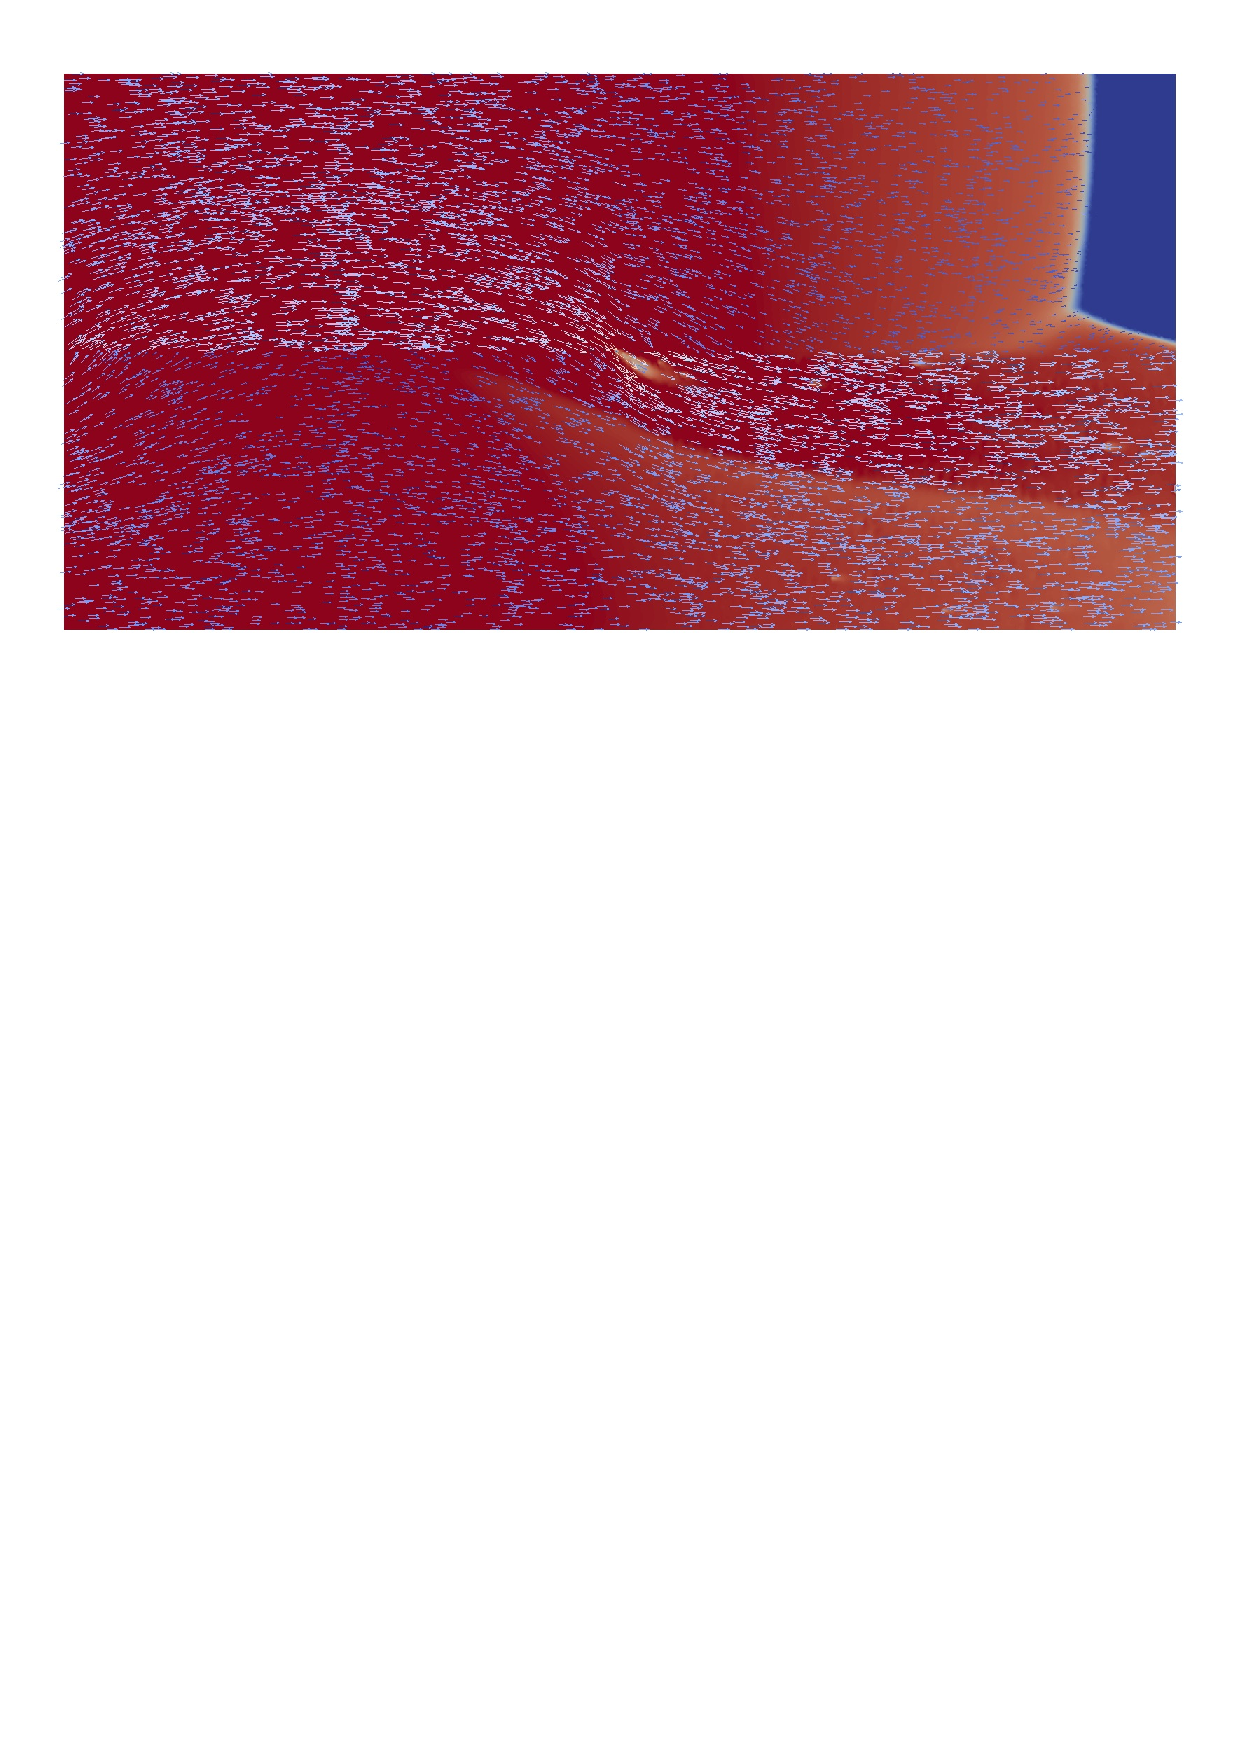
\includegraphics[width=.50\textwidth]{./Pics1/DaweGrattoni_Experiment/CrossFlow_d275b} 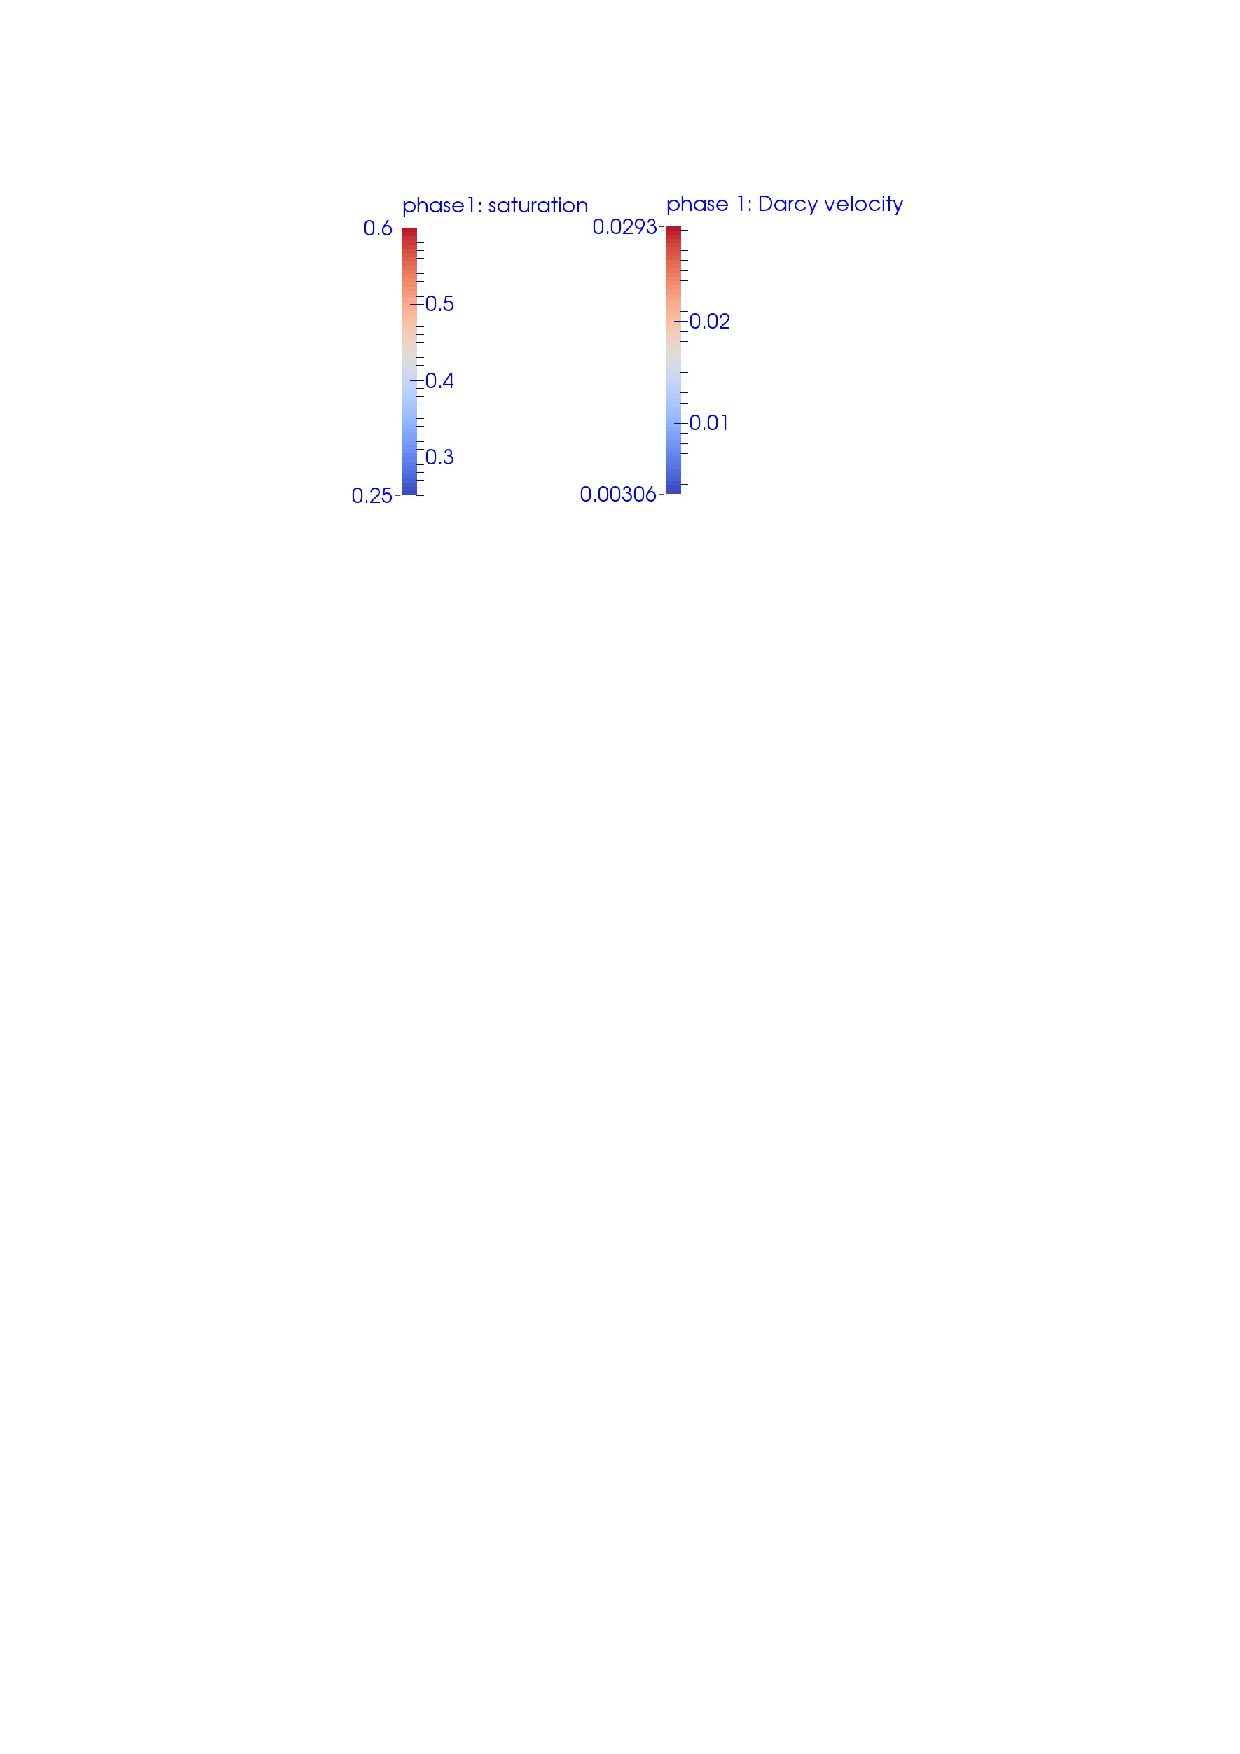
\includegraphics[width=.50\textwidth]{./Pics1/DaweGrattoni_Experiment/legendb} }
       \vspace{0.cm}
    }  
\caption{Model validation of fluid displacement in heterogeneous porous media ({\it VR}=1): Snapshots of wetting fluid saturation overlapped with Darcy velocity over t=39.70 time-units. The domain is divided in four subdomains with permeabilities of $\mathbf{K}_{1}=2.5$ and $\mathbf{K}_{2}=1$. The domain is discretised with 37872 \PN[1]{2} triangular elements. }
\label{DaweGrattoniExperiment_b}
  \end{figure}
\end{landscape}
\clearpage


%%%%
%%%%  FIGURE 
%%%%
\begin{figure}[h]
  \hbox{\hspace{2cm}
  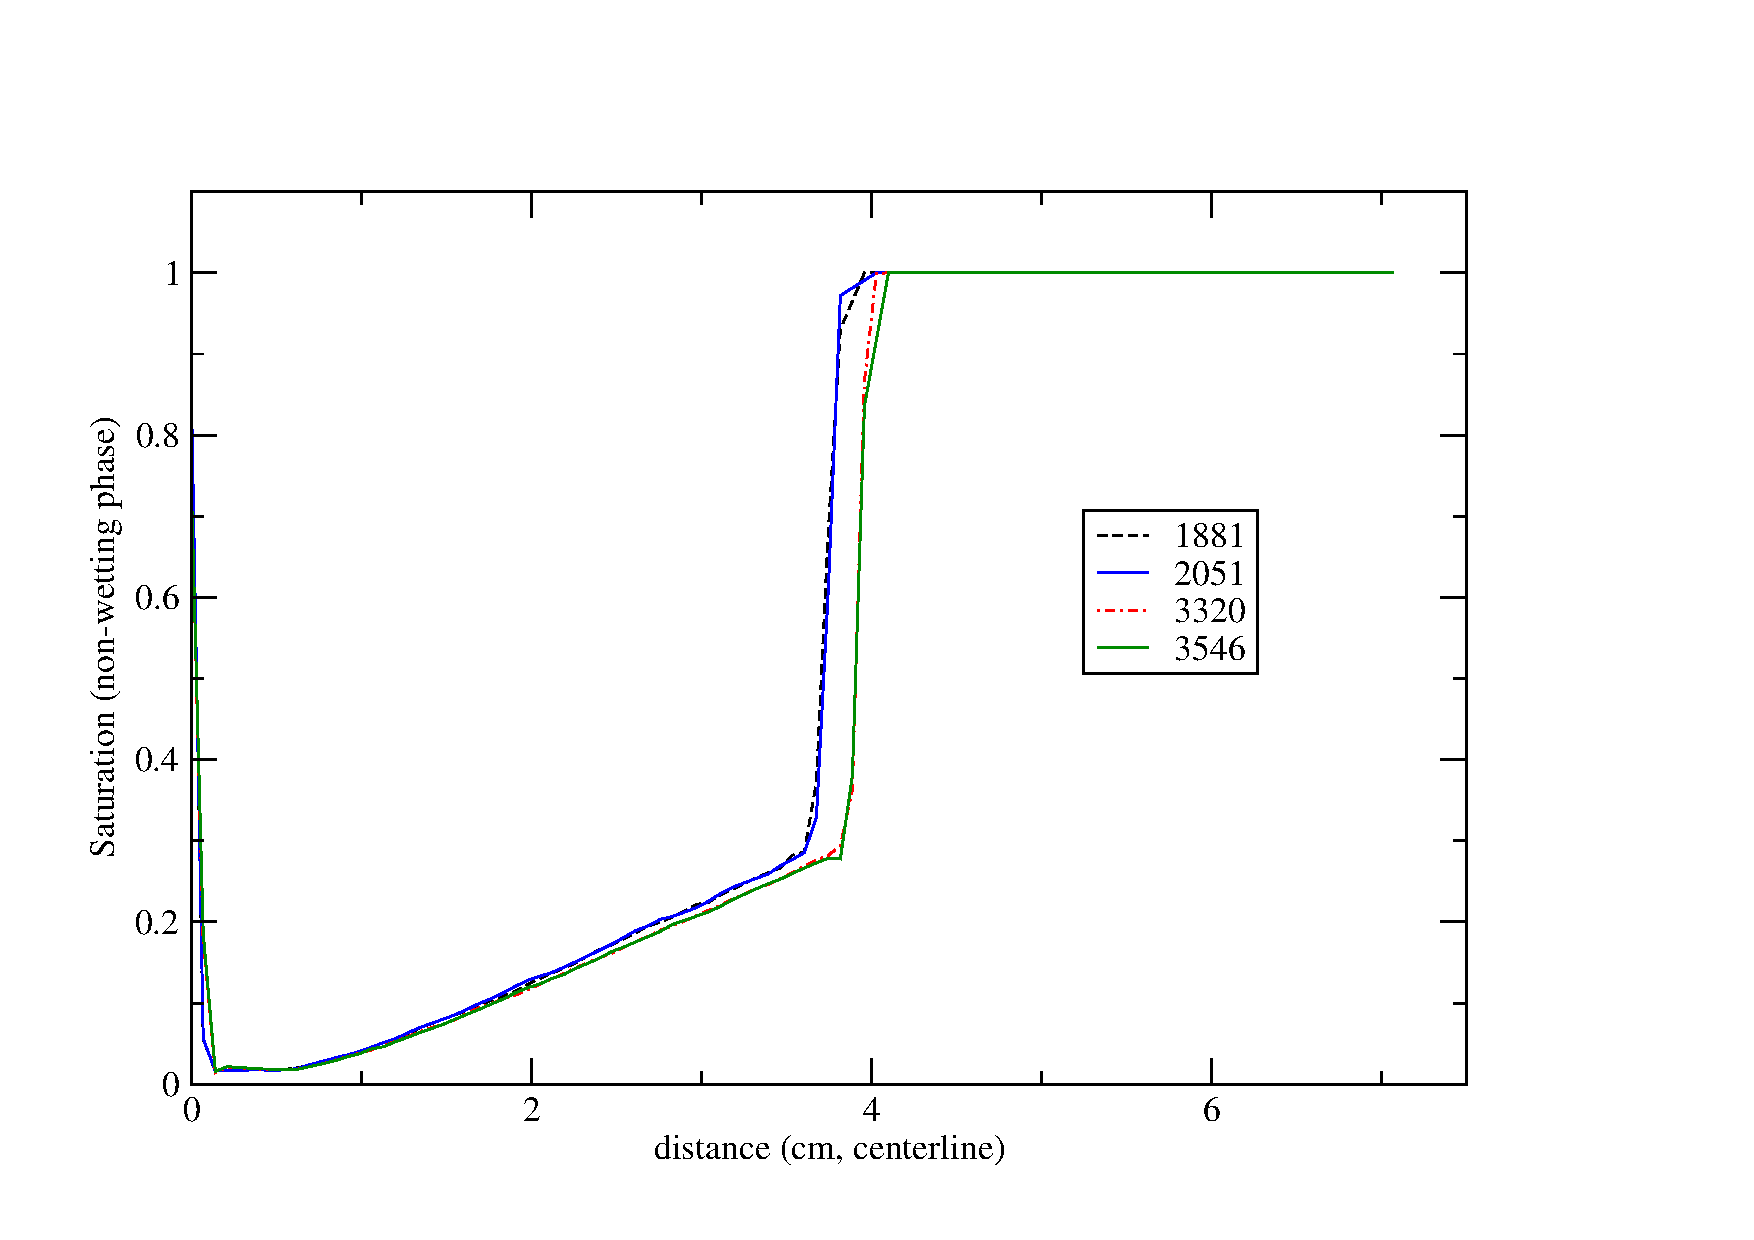
\includegraphics[width=0.75\textwidth]{./Pics1/Saffman_homogeneous/MeshIndependence.pdf}}
  \caption{Mesh convergence analysis for Hele-Shaw cells flow simulations (VR=1): non-wetting phase saturation profiles through a center-line across the domain (diagonal) with grid resolution ranging from 1881 to 3546 \PN[1]{2} triangular elements. }
\label{fig:MeshDependenceAnalysis}
\end{figure}
\clearpage

%%%%
%%%%  FIGURE
%%%%
\begin{landscape}
\begin{figure}[ht] 
\vbox{\vspace{-1cm}
\hbox{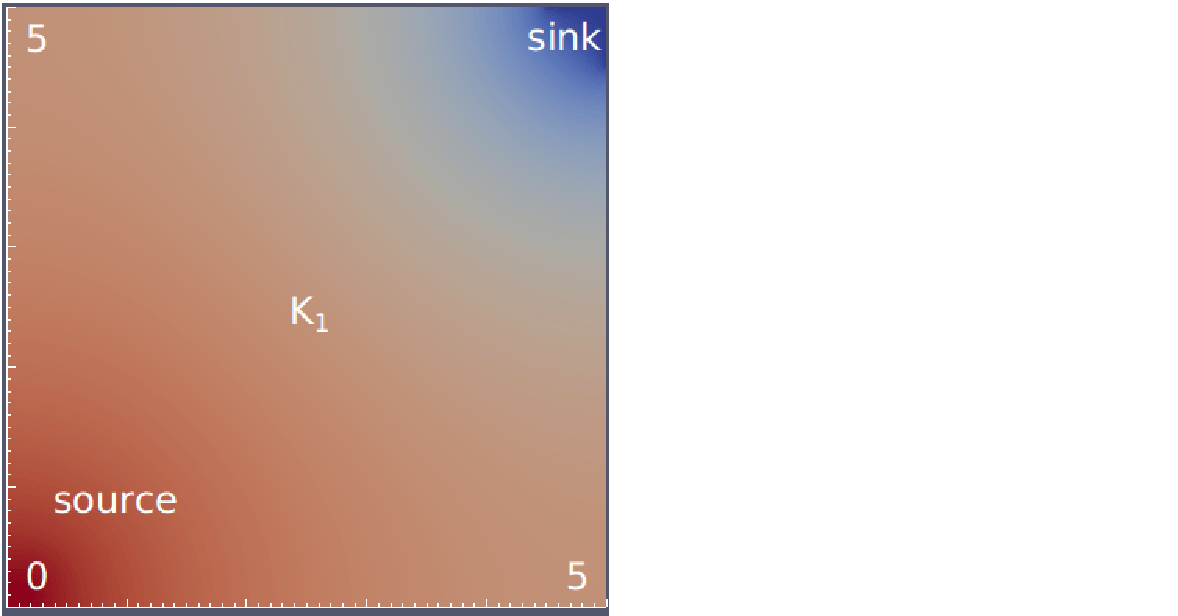
\includegraphics[width=.37\textwidth]{./Pics1/Saffman_homogeneous_MR3/saffman_homo_fixed_2b.pdf}
%\hbox{\includegraphics[width=.37\textwidth]{./Pics1/Saffman_homogeneous_MR3/saffman_homo_fixed_2.pdf}
      \includegraphics[width=.37\textwidth]{./Pics1/Saffman_homogeneous_MR3/saffman_homo_fixed_250.pdf}
      \includegraphics[width=.37\textwidth]{./Pics1/Saffman_homogeneous_MR3/saffman_homo_fixed_1000.pdf}}
\vspace{0.cm}
\hbox{\hspace{2.5cm} (a) schematics \hspace{3.cm} (b) t=0.87s \hspace{2.75cm} (c) t=3.54s}
\vspace{0.5cm}
\hbox{
      \includegraphics[width=.38\textwidth]{./Pics1/Saffman_homogeneous_MR3/saffman_homo_fixed_2500.pdf}
      \includegraphics[width=.38\textwidth]{./Pics1/Saffman_homogeneous_MR3/saffman_homo_fixed_3500.pdf} 
      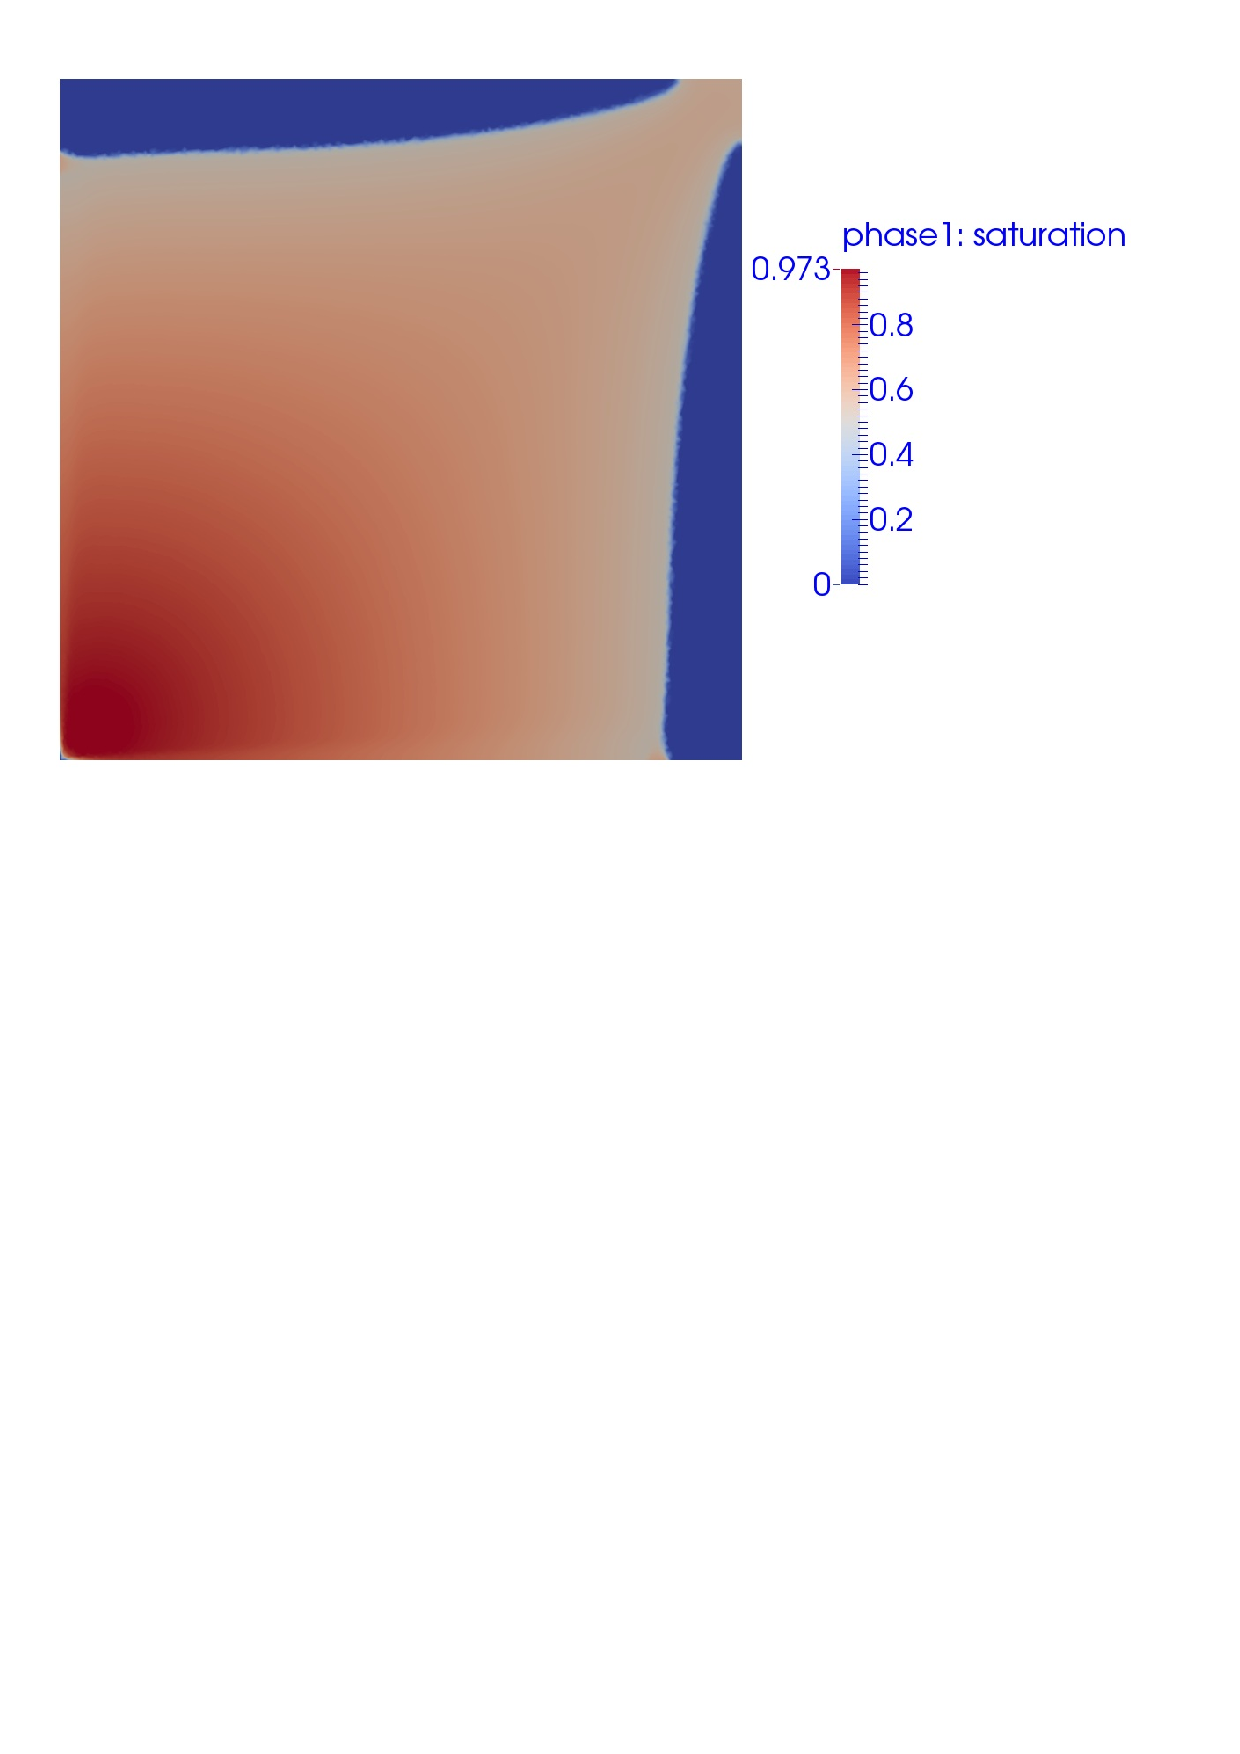
\includegraphics[width=.6\textwidth]{./Pics1/Saffman_homogeneous_MR3/saffman_homo_fixed_d5803_endb.pdf}}
      %\includegraphics[width=.66\textwidth]{./Pics1/Saffman_homogeneous_MR3/saffman_homo_fixed_end.pdf}}
\vspace{0.cm}
\hbox{ \hspace{1.cm} (d) t=8.86s \hspace{3.0cm} (e) t=12.41s   \hspace{4.0cm} (f) t=17.95s}
\vspace{0.cm}
}   
\caption{Simulated flow in a Hele-Shaw cell $\left(\text{{\it VR}=3, {\bf K}=10}^{-10}\text{cm}^{2}\right)$: (a) schematics of the HS cell indicating source and sink regions along with dimensions (in cm); (b-f) snapshots of wetting phase saturation showing flow profile as the simulation evolves. The domain was discretised with $26313$ \PN[1]{2} triangular elements.}
\label{fig:homoheleshaw_VN3}
\end{figure}
\end{landscape}
\clearpage



%%%%
%%%%  FIGURE
%%%%
\begin{landscape}
\begin{figure}[ht] 
\vbox{\vspace{-1cm}
%\hbox{\includegraphics[width=.9\textwidth, height=0.5\textwidth]{./Pics1/Saffman_homogeneous_VR10/ST_Homog_VR10_D201c.pdf}
%\hspace{0.5cm}      
      %\includegraphics[width=.5\textwidth]{./Pics1/Saffman_homogeneous_VR10/ST_Homog_VR10_D1001c.pdf}}
\hbox{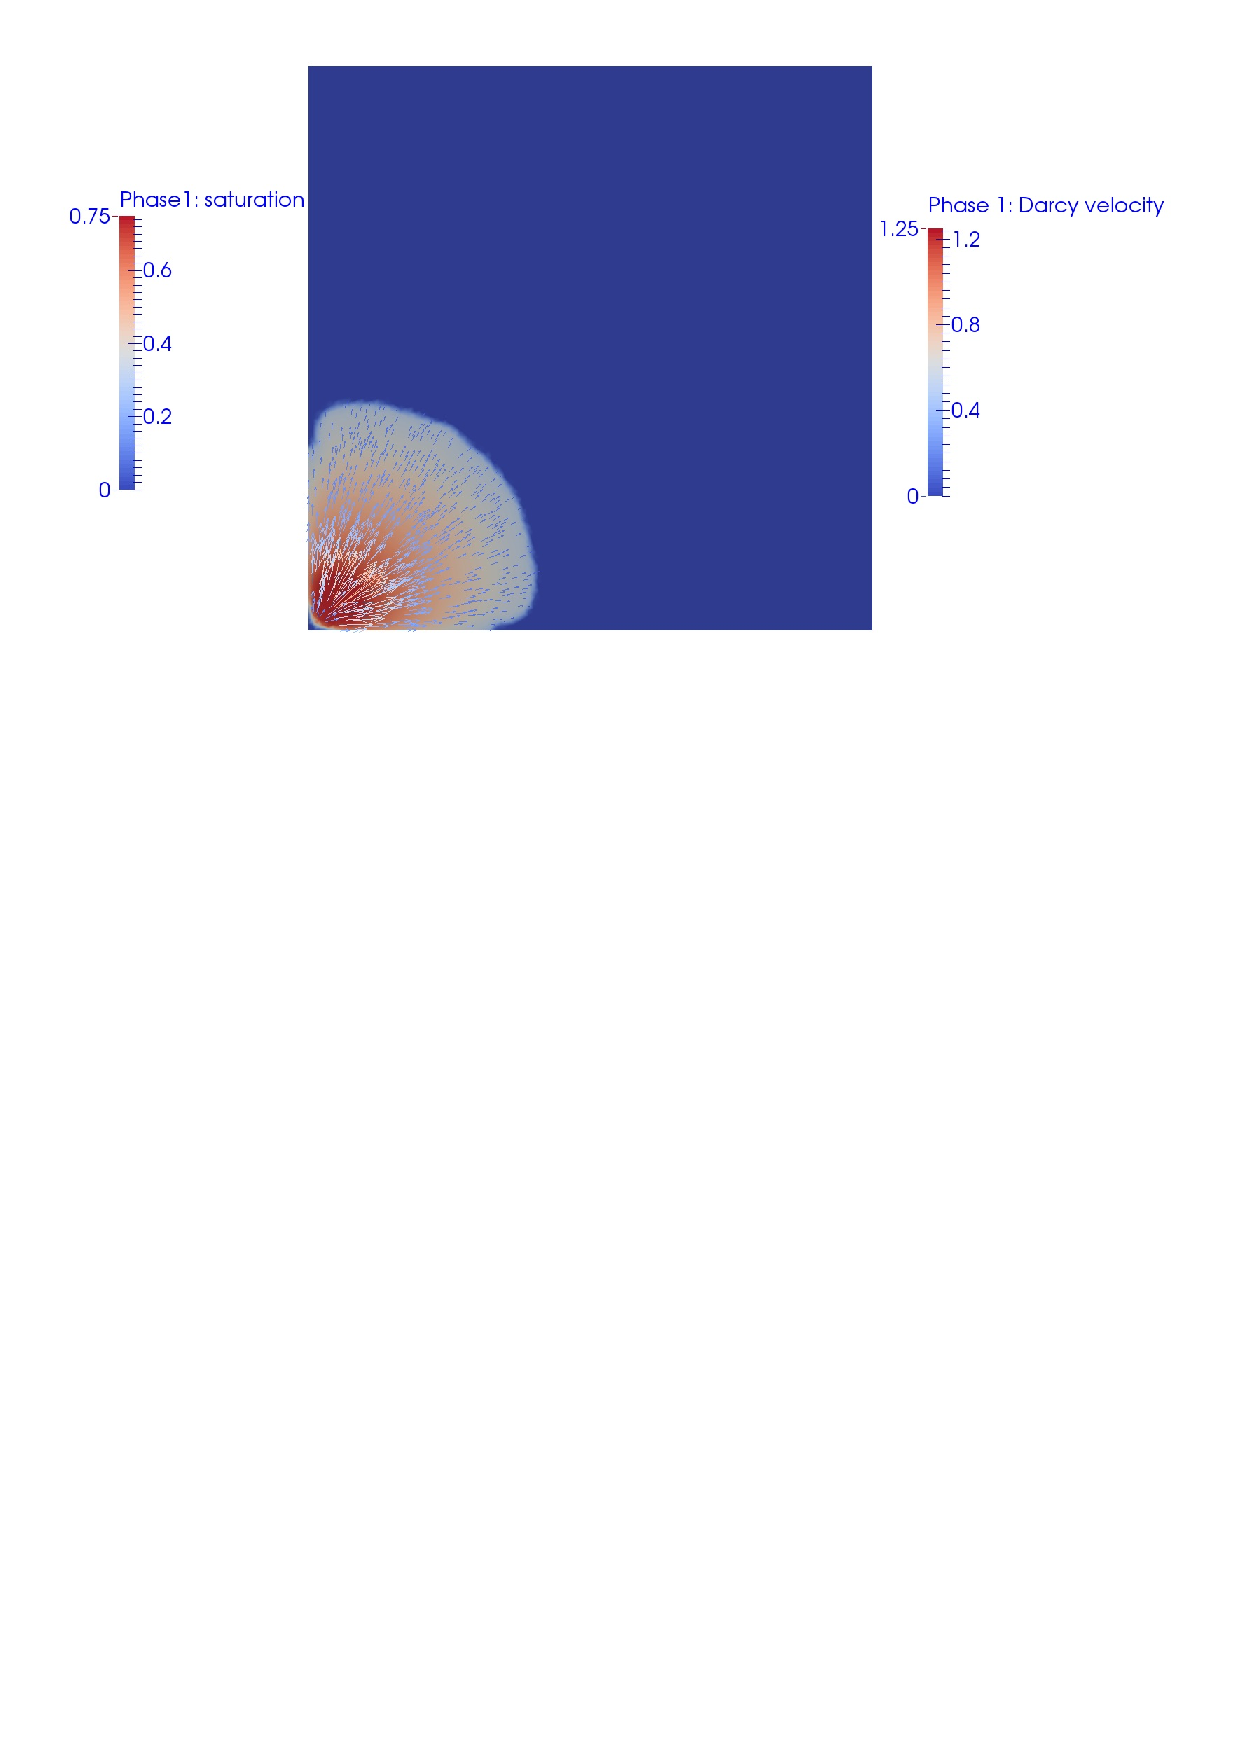
\includegraphics[width=\textwidth]{./Pics1/Saffman_homogeneous_VR10/ST_Homog_VR10_D1001cbd.pdf}
      \includegraphics[width=.51\textwidth]{./Pics1/Saffman_homogeneous_VR10/ST_Homog_VR10_D2001c.pdf}}
\vspace{0.cm}
\hbox{\hspace{5.cm} (a) t=3.43s  \hspace{8.cm} (b) t=6.92s}
\vspace{0.5cm}
\hbox{\hspace{3cm}
      %\includegraphics[width=.51\textwidth]{./Pics1/Saffman_homogeneous_VR10/ST_Homog_VR10_D2001c.pdf}
      \includegraphics[width=.5\textwidth]{./Pics1/Saffman_homogeneous_VR10/ST_Homog_VR10_D2201c.pdf}
      \hspace{4cm}\includegraphics[width=.51\textwidth]{./Pics1/Saffman_homogeneous_VR10/ST_Homog_VR10_D3001c.pdf}}
\vspace{0.cm}
\hbox{ \hspace{5.cm} (c) t=7.61s \hspace{8.cm} (d)t=10.00s}
\vspace{0.cm}
}   
\caption{Simulated flow in a Hele-Shaw cell $\left(\text{{\it VR}=10, {\bf K}=10}^{-10}\text{cm}^{2}\right)$: snapshots of overlapped wetting phase saturation and velocity vectors $\left(\text{in cm.s}^{-1}\right)$ showing flow profile as the simulation evolves. The domain was discretised with $26313$ \PN[1]{2} triangular elements.}
\label{fig:homoheleshaw_VN10}
\end{figure}
\end{landscape}
\clearpage

%%%%
%%%%  FIGURE
%%%%
\begin{landscape}
\begin{figure}[ht] 
\vbox{\vspace{-1cm}
%\hbox{\includegraphics[width=.8\textwidth, height=0.5\textwidth]{./Pics1/Saffman_homogeneous_VR150/ST_Homog_VR150_D300bcpdf}
\hbox{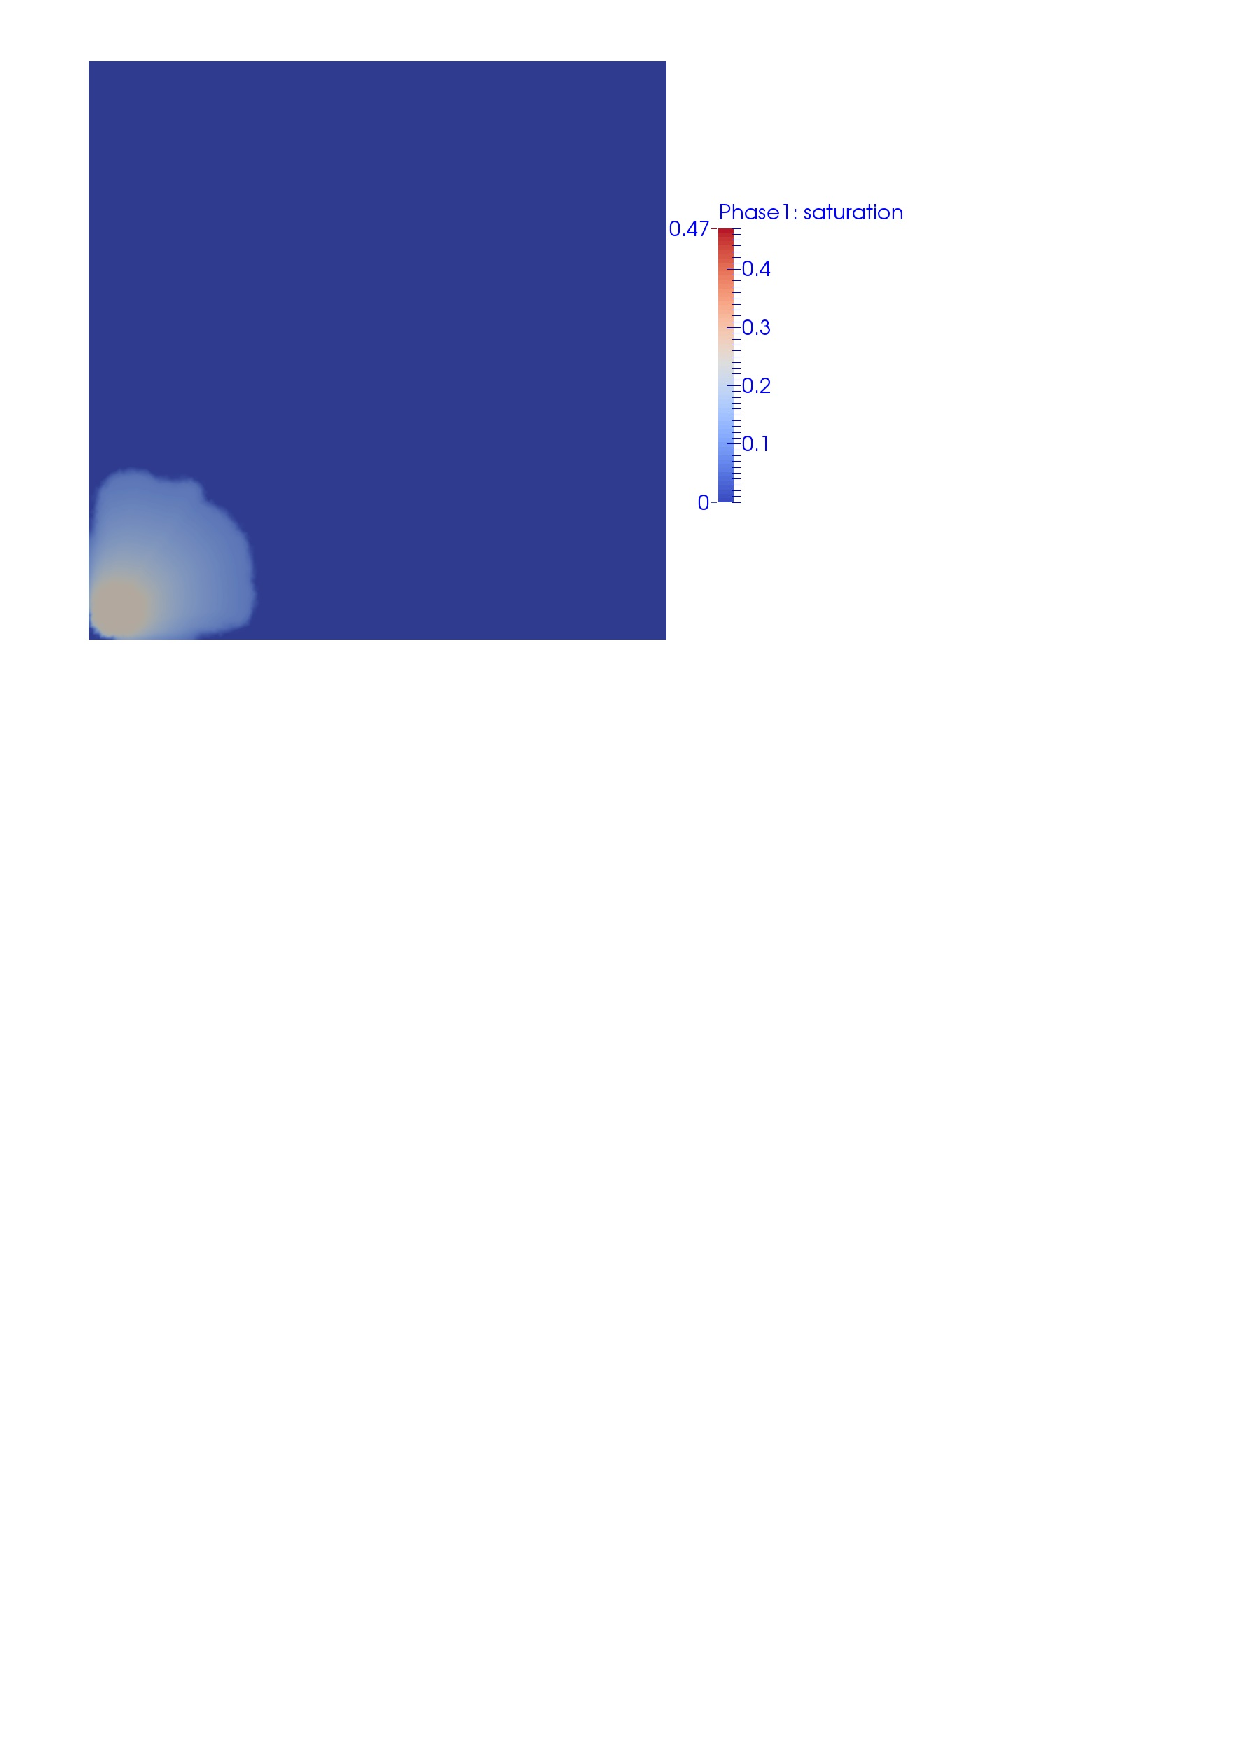
\includegraphics[width=.7\textwidth]{./Pics1/Saffman_homogeneous_VR150/ST_Homog_VR150_D300bcd.pdf}
\hspace{0.5cm}      
      \includegraphics[width=.5\textwidth]{./Pics1/Saffman_homogeneous_VR150/ST_Homog_VR150_D1600b.pdf}}
\vspace{0.cm}
\hbox{\hspace{5.cm} (a) t=0.27s \hspace{8.cm} (b) t=0.94s }
\vspace{0.5cm}
\hbox{
      \includegraphics[width=.5\textwidth]{./Pics1/Saffman_homogeneous_VR150/ST_Homog_VR150_D2700b.pdf}
      \includegraphics[width=.5\textwidth]{./Pics1/Saffman_homogeneous_VR150/ST_Homog_VR150_D4000b.pdf}
      \includegraphics[width=.51\textwidth]{./Pics1/Saffman_homogeneous_VR150/ST_Homog_VR150_D7000b.pdf}}
\vspace{0.cm}
\hbox{ \hspace{2.cm} (c) t=1.32s \hspace{4.5cm} (d) t=1.70s \hspace{5.cm} (e)t=2.31s}
\vspace{0.cm}
}   
\caption{Simulated flow in a Hele-Shaw cell $\left(\text{{\it VR}=150, {\bf K}=10}^{-10}\text{cm}^{2}\right)$: snapshots of wetting phase saturation showing flow profile as the simulation evolves. The domain was discretised with $26313$ \PN[1]{2} triangular elements.}
\label{fig:homoheleshaw_VN150}
\end{figure}
\end{landscape}
\clearpage


%%%%
%%%%  FIGURE
%%%%
\begin{figure}[ht]
\vbox{
\hbox{\includegraphics[width=.5\textwidth]{./Pics1/Saffman_homogeneous_VR10/ST_Homog_VR10_D2201_W2b.pdf}
       \includegraphics[width=.5\textwidth]{./Pics1/Saffman_homogeneous_VR150/ST_Homog_VR150_D5003_W2b.pdf}}
\hbox{\hspace{0.25cm} (a) {\it VR}=10 (homogeneous) \hspace{1.5cm} (b) {\it VR}=150 (homogeneous) }
\vspace{0.5cm}
\hbox{\includegraphics[width=.5\textwidth]{./Pics1/Saffman_heterogeneous_VR10/ST_Heterog_VR10_D11000_W2b.pdf}
       \includegraphics[width=.5\textwidth]{./Pics1/Saffman_heterogeneous_VR150/ST_Heterog_VR150_D6500_W2b.pdf}}
\hbox{\hspace{0.25cm} (c) {\it VR}=10 (heterogeneous) \hspace{1.5cm} (d) {\it VR}=150 (heterogeneous) }
}
\caption{Isosurfaces of simulated flows in Hele-Shaw cells with viscosity ratios of 10 (a and c) and 150 (b and d). Top and bottom rows describe simulations performed with constant $\left(\text{\ie homogeneous with }\textbf{K}\text{ = 10}^{-10}\text{ cm}^{2}\right)$ and randomly distributed (\ie heterogeneous, Fig.~\ref{fig:HeleShawHeter_VR10}a) permeabilities. Width of largest fingers for homogeneous cases are approximately $0.70$ and $0.90$cm (\textit{VR}=$10$ and \textit{VR}=$150$, respectively), whereas for heterogeneous cases are $0.56$ and $0.40$cm. Results for homogeneous cases are in good agreement with values obtained from \citet{guan_2003}'s analytic solution.}
\label{fig:homoheleshaw_VN10_VN150}
\end{figure}
\clearpage




%%%
%%% FIGURE XXXXXX
%%%
\begin{landscape}
  \begin{figure}[ht]
  \vbox{\vspace{-.5cm}
      \hbox{\includegraphics[width=.4\textwidth]{./Pics1/Saffman_heterogeneous/saffman_heter_fixed_1.pdf}
            %\includegraphics[width=.55\textwidth, height=.4\textwidth]{./Pics1/Saffman_heterogeneous_VR10/ST_Heterog_VR10_D200Hb.pdf} 
            \includegraphics[width=.57\textwidth]{./Pics1/Saffman_heterogeneous_VR10/ST_Heterog_VR10_D200Hbcd.pdf} 
            \includegraphics[width=.42\textwidth]{./Pics1/Saffman_heterogeneous_VR10/ST_Heterog_VR10_D900Hb.pdf} }
      \hbox{\hspace{1.0cm} (a) permeability map \hspace{3.cm} (b) t=0.19s \hspace{4.0cm} (c) t=0.63s}
      \vspace{0.5cm}
      \hbox{\includegraphics[width=.45\textwidth]{./Pics1/Saffman_heterogeneous_VR10/ST_Heterog_VR10_D5000Hb.pdf}
            \includegraphics[width=.45\textwidth]{./Pics1/Saffman_heterogeneous_VR10/ST_Heterog_VR10_D8000Hb.pdf}
            \includegraphics[width=.45\textwidth]{./Pics1/Saffman_heterogeneous_VR10/ST_Heterog_VR10_D13800Hb.pdf} }
      \hbox{\hspace{2.cm} (d) t=3.41s \hspace{3.5cm} (e) t= 5.54s\hspace{4.5cm} (f) t=9.77s }}
\caption{Simulated flow in a modified Hele-Shaw cell with {\it VR}=10: (a) permeability distribution $\left(\text{10}^{-10}\le\mathbf{K}_{1}\le\text{5}\times\text{10}^{-10}\right.$, {\bf K}$_{2}$=10$^{-10}$, 10$^{-11}\le\mathbf{K}_{3}\le$ 5$\times$10$^{-10}$ and 10$^{-12}\le\mathbf{K}_{4}\le$ 5$\times$10$\left.^{-10}\text{ cm}^{2}\right)$; (b-f) snapshots of saturation profile during 9.77 seconds of simulation. The domain was discretised with 26313 \PN[1]{2} element-pairs.}
\label{fig:HeleShawHeter_VR10}
\end{figure}
\end{landscape}
\clearpage


%%%
%%% FIGURE XXXXXX
%%%
\begin{landscape}
  \begin{figure}[ht]
  \vbox{\vspace{-.5cm}
      %\hbox{\includegraphics[width=.65\textwidth, height=.46\textwidth]{./Pics1/Saffman_heterogeneous_VR150/ST_Heterog_VR150_D200Hb.pdf} 
      \hbox{\includegraphics[width=.65\textwidth]{./Pics1/Saffman_heterogeneous_VR150/ST_Heterog_VR150_D200Hbcd.pdf} 
            \includegraphics[width=.45\textwidth]{./Pics1/Saffman_heterogeneous_VR150/ST_Heterog_VR150_D500Hb.pdf}
            \includegraphics[width=.45\textwidth]{./Pics1/Saffman_heterogeneous_VR150/ST_Heterog_VR150_D800Hb.pdf} }
      \hbox{\hspace{2.0cm} (a) t=0.10s \hspace{6.cm} (b) t=0.24s \hspace{4.cm} (c) t=0.37s}
      \vspace{0.5cm}
      \hbox{\hspace{.5cm} \includegraphics[width=.45\textwidth]{./Pics1/Saffman_heterogeneous_VR150/ST_Heterog_VR150_D1500Hb.pdf}
            \includegraphics[width=.45\textwidth]{./Pics1/Saffman_heterogeneous_VR150/ST_Heterog_VR150_D5000Hb.pdf}
            \includegraphics[width=.45\textwidth]{./Pics1/Saffman_heterogeneous_VR150/ST_Heterog_VR150_D8000Hb.pdf} }
      \hbox{\hspace{3.cm} (d) t=0.59s \hspace{3.cm} (e) t= 1.61s\hspace{4.cm} (f) t=2.50s }}
\caption{Simulated flow in a modified Hele-Shaw cell with {\it VR}=150: snapshots of saturation profile during 2.50 seconds of simulation. Permeability distribution used in this simulation was the same as shown in Fig.~\ref{fig:HeleShawHeter_VR10}a. The domain was discretised with 26313 \PN[1]{2} element-pairs.}
\label{fig:HeleShawHeter_VR150}
\end{figure}
\end{landscape}
\clearpage



%%%
%%% FIGURE XXXXXX 
%%%
\begin{landscape}
  \begin{figure}[ht]
  \vbox{\vspace{-.5cm}
      %\hbox{\includegraphics[width=.65\textwidth, height=.45\textwidth]{./Pics1/Saffman_new/ST_Heterog_50.pdf} 
      \hbox{\includegraphics[width=.65\textwidth]{./Pics1/Saffman_new/ST_Heterog_50bcd.pdf} 
            \includegraphics[width=.45\textwidth]{./Pics1/Saffman_new/ST_Heterog_500.pdf}
            \includegraphics[width=.45\textwidth]{./Pics1/Saffman_new/ST_Heterog_1000.pdf} }
      \hbox{\hspace{2.0cm} (a) t=0.07s \hspace{6.cm} (b) t=0.96s \hspace{4.cm} (c) t=2.0s}
      \vspace{0.5cm}
      \hbox{\hspace{.5cm} \includegraphics[width=.45\textwidth]{./Pics1/Saffman_new/ST_Heterog_1500.pdf}
            \includegraphics[width=.45\textwidth]{./Pics1/Saffman_new/ST_Heterog_1800.pdf}
            \includegraphics[width=.45\textwidth]{./Pics1/Saffman_new/ST_Heterog_2180.pdf} }
      \hbox{\hspace{3.cm} (d) t=2.7s \hspace{3.cm} (e) t= 3.13s\hspace{4.cm} (f) t=3.42s }}
\caption{Simulated flow in a modified Hele-Shaw cell with {\it VR}=150: snapshots of saturation profile. Permeability distribution used in this simulation was the same as shown in Fig.~\ref{fig:HeleShawHeter_VR10}a. The domain was discretised with 3734 \PN[1]{2} element-pairs.}
\label{fig:HeleShawHeter_VR150_coarse}
\end{figure}
\end{landscape}
\clearpage



%%%%
%%%%  FIGURE
%%%%
\begin{figure}[ht] 
\vbox{
\vspace{-.5cm}
%\hbox{\hspace{4.0cm}
%\includegraphics[width=.75\textwidth]{./Pics/map_of_boundaries.pdf} 
%}
%\vspace{0.0cm}
%\hbox{\hspace{6.5cm} (a) Schematics of the domain
%}
%\vspace{0.25cm}
%\hbox{\hspace{4.0cm}
%\includegraphics[width=\textwidth]{./Pics1/Four_regions_coarse_MeshPermeability}
\hbox{\hspace{.8cm}
\includegraphics[width=\textwidth, height=0.45\textwidth]{./Pics1/Section4_4/Sketch_5Regions.pdf}}
\vspace{-.5cm}
\hbox{\hspace{3.5cm} (a) Sketch}
\hbox{\hspace{1cm}
\includegraphics[width=\textwidth, height=0.45\textwidth]{./Pics1/Section4_4/Five_regions_adapt_MeshPerm.pdf}}
\vspace{-1.0cm}
\hbox{\hspace{3.5cm} (b) Permeability mapping ({\bf K})}
\vspace{0.0cm}
\hbox{\hspace{1cm}
\includegraphics[width=\textwidth, height=0.45\textwidth]{./Pics1/Section4_4/Five_regions_adapt_MeshSat1.pdf}}
\vspace{-1.0cm}
\hbox{\hspace{3.5cm} (c) Initial saturation distribution}}
%}
%\vspace{0.0cm}
%\hbox{\hspace{4cm} (b) Permeability distribution for coarse mesh simulation     
%}
%}     
\caption{Impact of mesh resolution on capturing flow instabilities: (a) sketch of the computational domain (dimensions in unit-length); (b) permeability, and; (c) initial saturation and  mesh resolution used in the simulations performed in Section~\ref{section:results_hete_fix_adapt}. There are 13068 \PN[1]{2} element-pairs in the domain.}
\label{fig:testcase_heter_domain}
\end{figure}
\clearpage



%%%
%%% FIGURE XXXXXX
%%%
  \begin{figure}[ht]
  \vbox{\vspace{-1.cm}
      \hbox{\includegraphics[width=.45\textwidth]{./Pics1/Section4_4/5r_po_left_inlet_D0b.pdf}
            \includegraphics[width=.45\textwidth]{./Pics1/Section4_4/5r_po_left_inlet_D250b.pdf}} 
            %\includegraphics[width=.45\textwidth]{./Pics1/Section4_4/5r_po_left_inlet_D350b.pdf}}
      \vspace{-.1cm}\hbox{\hspace{2.cm}(a) t=0.00 \hspace{4cm} (f) t= 0.35}\vspace{-.1cm}
      \hbox{\includegraphics[width=.45\textwidth]{./Pics1/Section4_4/5r_po_left_inlet_D100b.pdf} 
            \includegraphics[width=.45\textwidth]{./Pics1/Section4_4/5r_po_left_inlet_D700b.pdf}}
      \vspace{-.1cm}\hbox{\hspace{2.cm}(b) t=0.10 \hspace{4cm} (g) t= 0.70}\vspace{-.1cm}
      \hbox{\includegraphics[width=.45\textwidth]{./Pics1/Section4_4/5r_po_left_inlet_D150b.pdf} 
            \includegraphics[width=.45\textwidth]{./Pics1/Section4_4/5r_po_left_inlet_D1000b.pdf}}
      \vspace{-.1cm}\hbox{\hspace{2.cm}(c) t=0.15 \hspace{4cm} (h) t= 1.00}\vspace{-.1cm}
      \hbox{\includegraphics[width=.45\textwidth]{./Pics1/Section4_4/5r_po_left_inlet_D200b.pdf} 
            \includegraphics[width=.45\textwidth]{./Pics1/Section4_4/5r_po_left_inlet_D1500b.pdf}}
      \vspace{-.1cm}\hbox{\hspace{2.cm}(d) t=0.20 \hspace{4cm} (i) t= 1.50}\vspace{-.1cm}
      \hbox{\includegraphics[width=.45\textwidth]{./Pics1/Section4_4/5r_po_left_inlet_D350b.pdf}}
      %\hbox{\includegraphics[width=.45\textwidth]{./Pics1/Section4_4/5r_po_left_inlet_D250b.pdf}}
      \vspace{-.1cm}\hbox{\hspace{2.cm}(e) t=0.25}\vspace{-.1cm}}
\caption{Impact of mesh resolution on capturing flow instabilities: snapshots of saturation field through 1.50 unit-time of numerical simulation performed with fixed mesh (i) of 13068 elements and {\it VR}=10.}
\label{fig:5regions_fixedmesh}
\end{figure}
\clearpage



%%%
%%% FIGURE XXXXXX
%%%
  \begin{figure}[ht]
  \vbox{\vspace{-2.cm}
      \hbox{\includegraphics[width=.45\textwidth]{./Pics1/Section4_4/5r_po_left_inlet_adapt_D0b.pdf} 
            \includegraphics[width=.45\textwidth]{./Pics1/Section4_4/5r_po_left_inlet_adapt_D350b.pdf}}
      \vspace{-.1cm}\hbox{\hspace{2.cm}(a) t=0.00 \hspace{4cm} (f) t= 0.35}\vspace{-.1cm}
      \hbox{\includegraphics[width=.45\textwidth]{./Pics1/Section4_4/5r_po_left_inlet_adapt_D100b.pdf} 
            \includegraphics[width=.45\textwidth]{./Pics1/Section4_4/5r_po_left_inlet_adapt_D700b.pdf}}
      \vspace{-.1cm}\hbox{\hspace{2.cm}(b) t=0.10 \hspace{4cm} (g) t= 0.70}\vspace{-.1cm}
      \hbox{\includegraphics[width=.45\textwidth]{./Pics1/Section4_4/5r_po_left_inlet_adapt_D150b.pdf} 
            \includegraphics[width=.45\textwidth]{./Pics1/Section4_4/5r_po_left_inlet_adapt_D1000b.pdf}}
      \vspace{-.1cm}\hbox{\hspace{2.cm}(c) t=0.15 \hspace{4cm} (h) t= 1.00}\vspace{-.1cm}
      \hbox{\includegraphics[width=.45\textwidth]{./Pics1/Section4_4/5r_po_left_inlet_adapt_D200b.pdf} 
            \includegraphics[width=.45\textwidth]{./Pics1/Section4_4/5r_po_left_inlet_adapt_D1500b.pdf}}
      \vspace{-.1cm}\hbox{\hspace{2.cm}(d) t=0.20 \hspace{4cm} (i) t= 1.50}\vspace{-.1cm}
      \hbox{\includegraphics[width=.45\textwidth]{./Pics1/Section4_4/5r_po_left_inlet_adapt_D250b.pdf}}
      \vspace{-.1cm}\hbox{\hspace{2.cm}(e) t=0.25}\vspace{-.1cm}}
\caption{Impact of mesh resolution on capturing flow instabilities: snapshots of saturation field through 1.50 unit-time of numerical simulation performed with adaptive mesh and {\it VR}=10.}
\label{fig:5regions_adaptmesh}
\end{figure}
\clearpage



%%%%
%%%%  FIGURE
%%%%
\begin{figure}[ht] 
\includegraphics[width=\textwidth]{./Pics1/Section4_4/Five_regions_adapt_PlotTimeNodesElements.pdf}
\caption{Impact of mesh resolution on capturing flow instabilities: total number of elements (red) and nodes (blue) for simulations performed with fixed (dotted line) and adaptive (full line) mesh. }
\label{fig:5regions_plottimenodeselements}
\end{figure}



%%%
%%% FIGURE XXXXXX
%%%
%\begin{landscape}
  \begin{figure}[ht]
  \vbox{\vspace{-.5cm}
      \hbox{\includegraphics[width=.5\textwidth, height=0.3\textwidth,clip]{./Pics1/Section4_4/5r_po_left_inlet_D250_meshb.pdf}
            \includegraphics[width=.5\textwidth, height=0.33\textwidth,clip]{./Pics1/Section4_4/5r_po_left_inlet_adapt_D250_edb.pdf} }
      \vspace{-0.cm}\hbox{\hspace{4.5cm}(a) fixed and adaptive mesh  }\vspace{-0.cm}
      %\hbox{\includegraphics[width=.5\textwidth]{./Pics1/Section4_4/5r_po_left_inlet_adapt_D251_vel1b.pdf}
      %      \includegraphics[width=.5\textwidth]{./Pics1/Section4_4/5r_po_left_inlet_adapt_D251_vel2b.pdf} }
      %\vspace{-0.cm}\hbox{\hspace{1cm}(b) Darcy velocity (phase 1) \hspace{1cm}(c) Darcy velocity (phase 2) }\vspace{0.cm}
      \hbox{ \includegraphics[width=.5\textwidth, height=0.3\textwidth,clip]{./Pics1/Section4_4/5r_po_left_inlet_D251_Zoom1b.pdf}
             \includegraphics[width=.5\textwidth, height=0.3\textwidth,clip]{./Pics1/Section4_4/5r_po_left_inlet_adapt_D251_Zoom1b.pdf} }
      \vspace{-0.cm}\hbox{\hspace{4.5cm}(b) Zoom on region {\it A}  }\vspace{-0.cm}
      \hbox{ \includegraphics[width=.5\textwidth, height=0.3\textwidth,clip]{./Pics1/Section4_4/5r_po_left_inlet_D251_Zoom2b.pdf}
             \includegraphics[width=.5\textwidth, height=0.3\textwidth,clip]{./Pics1/Section4_4/5r_po_left_inlet_adapt_D251_Zoom2b.pdf}}
      \vspace{-0.cm}\hbox{\hspace{4.5cm}(c) Zoom on region {\it B}  }\vspace{-0.cm}}
\caption{Impact of mesh resolution on flow instabilities: capturing formation and growth of flow instabilities at fluid interfaces (t = 0.20) in two regions of the computational domain, {\it A} and {\it B}. Simulations were conducted with fixed (left-hand side) and adaptive meshes. }
\label{fig:5regions_AdaptZoom}
\end{figure}
%\end{landscape}
\clearpage



%%%
%%% FIGURE XXXXXX
%%%
\begin{figure}[ht]
\vbox{\vspace{-.5cm}
      \hbox{\includegraphics[width=\textwidth]{./Pics1/3D_Channel/Test_SlowNew_MeshPermeability.pdf} }}
\caption{3D channel flow: Permeability distribution within the computational domain, containing 235242 \PNDG[1]{1} tetrahedra element-pairs.}
\label{fig:3DChannel_PermMesh}
\end{figure}
\clearpage




%%%
%%% FIGURE XXXXXX
%%%
\begin{landscape}
\begin{figure}[ht]
  \vbox{\vspace{-.5cm}
      \hbox{\includegraphics[width=.6\textwidth]{./Pics1/3D_Channel/3D_channel_sat_30.pdf} 
            \includegraphics[width=.5\textwidth]{./Pics1/3D_Channel/3D_channel_sat_60.pdf}
            \includegraphics[width=.5\textwidth]{./Pics1/3D_Channel/3D_channel_sat_90.pdf} } 
      \hbox{\hspace{2.cm} (a) t=0.29s \hspace{5.cm} (b) t=0.56s \hspace{4.cm} (c) t=0.82s}
      \vspace{0.5cm}
      \hbox{\hspace{.5cm} 
            \includegraphics[width=.5\textwidth]{./Pics1/3D_Channel/3D_channel_sat_110.pdf}
            \includegraphics[width=.5\textwidth]{./Pics1/3D_Channel/3D_channel_sat_150.pdf}
            \includegraphics[width=.5\textwidth]{./Pics1/3D_Channel/3D_channel_sat_490.pdf} }
      \hbox{\hspace{2.cm} (d) t=1.00s \hspace{5.cm} (e) t=1.35s\hspace{4.cm} (f) t=3.50s  } }
\caption{3D channel flow (fixed mesh): saturation front evolving in time and space with preferential flow pathways through 3.50 seconds of numerical simulations. Preferential flow pathway can be readily noticed in these frames, mirroring permeability distribution. The domain was discretised with 235242 \PNDG[1]{1} elements.}
\label{fig:3DChannel_sat}
\end{figure}
\end{landscape}
\clearpage


%%%%
%%%%  FIGURE
%%%%
%\begin{landscape}
\begin{figure}[ht] 
\vbox{
\hbox{\hspace{0.5cm}
\includegraphics[width=1.0\textwidth]{./Pics1/3D_Channel/3D_channel_darcy_vel_planes_490_1_1.pdf} 
}
\vspace{-12.0cm}
\hbox{\hspace{6.0cm} (a)     
}
\hbox{\hspace{0.5cm}
\includegraphics[width=1.0\textwidth]{./Pics1/3D_Channel/3D_channel_darcy_vel_planes_30_1_1.pdf}
}
\vspace{-12.0cm}
\hbox{\hspace{6.0cm} (b)      
}
}     
\caption{3D channel flow (fixed mesh): XY and YZ planes showing wetting phase saturation overlapped with Darcy velocity vectors $\left(\text{in cm.s}^{-1}\right)$  at (a) t=$0.29$s and (b)t=$4.3$s.}
\label{fig:3DChannel_planes}
\end{figure}
%\end{landscape}
\clearpage



%%%
%%% FIGURE XXXXXX
%%%
\begin{landscape}
  \begin{figure}[ht]
  \vbox{\vspace{-.5cm}
      \hbox{\includegraphics[width=.55\textwidth, height=.45\textwidth]{./Pics1/3D_Channel/3D_Channel_Saturation1Isosurface_D30c.pdf} 
            \includegraphics[width=.5\textwidth]{./Pics1/3D_Channel/3D_Channel_Saturation1Isosurface_D60c.pdf}
            \includegraphics[width=.5\textwidth]{./Pics1/3D_Channel/3D_Channel_Saturation1Isosurface_D90c.pdf} }
      \hbox{\hspace{2.0cm} (a) t=0.29s \hspace{6.cm} (b) t=0.56s \hspace{4.cm} (c) t=0.82s}
      \vspace{0.5cm}
      \hbox{\hspace{.5cm} \includegraphics[width=.45\textwidth]{./Pics1/3D_Channel/3D_Channel_Saturation1Isosurface_D110c.pdf}
            \includegraphics[width=.45\textwidth]{./Pics1/3D_Channel/3D_Channel_Saturation1Isosurface_D150c.pdf}
            \includegraphics[width=.45\textwidth]{./Pics1/3D_Channel/3D_Channel_Saturation1Isosurface_D400c.pdf} }
      \hbox{\hspace{3.cm} (d) t=1.00s \hspace{3.cm} (e) t=1.35s\hspace{4.cm} (f) t=3.50s }}
\caption{3D channel flow (fixed mesh): Isosurfaces for wetted phase saturatioh ranging from 0.45 and 0.60 at the same instants of time of Fig.~\ref{fig:3DChannel_sat}. Preferential flow pathway can be readily noticed in (b) and (f). Fingers' formation and growth can be clearly noticed in (b)-(e). The domain was discretised with 235242 \PNDG[1]{1} elements.}
\label{fig:3DChannel_Isosurf}
\end{figure}
\end{landscape}
\clearpage


%%%%
%%%%  FIGURE
%%%%
\begin{landscape}
  \begin{figure}[ht] 
    \vbox{\vspace{0.cm}
        \hbox{\hspace{5.cm}
          \includegraphics[width=\textwidth]{./Pics1/3D_ChannelAdaptive/Test_SlowNewAdapt_288_Mesh_b} }
        \hbox{\hspace{10cm}(a)}
      \vspace{.5cm} 
         \hbox{\hspace{0.cm}
             \includegraphics[width=0.75\textwidth]{./Pics1/3D_ChannelAdaptive/Test_SlowNewAdapt_288_StreamLinesHoriz_b} 
      \hspace{.5cm} 
             \includegraphics[width=0.75\textwidth]{./Pics1/3D_ChannelAdaptive/Test_SlowNewAdapt_288_Isosurface_b} 
         }
        \hbox{\hspace{6cm}(b) \hspace{8cm}(c)}
    }
\caption{3D Channel (adaptive mesh): (a) Wetting fluid saturation overlapped with mesh; (b) streamlines and; (c) isosurfaces. All plots are shown at 3.78s (Fig.~\ref{fig:3DChannel_satvel_XYplanes_adapt}f). }
\label{fig:3DChannel_severalfields_adapt}
\end{figure}
\end{landscape}
\clearpage

%%%%
%%%%  FIGURE
%%%%
%\begin{landscape}
  \begin{figure}[ht] 
    \vbox{\vspace{0.cm}
        \hbox{\hspace{-3.cm}
            \includegraphics[width=.75\textwidth]{./Pics1/3D_ChannelAdaptive/Test_SlowNewAdapt_0_ContourPlotSlice_b} \hspace{-.5cm}
            \includegraphics[width=.70\textwidth]{./Pics1/3D_ChannelAdaptive/Test_SlowNewAdapt_20_ContourPlotSlice_b}}
        \hbox{\hspace{2cm}(a)\hspace{9cm}(b)}
        \hbox{\hspace{-3.cm}
            \includegraphics[width=.70\textwidth]{./Pics1/3D_ChannelAdaptive/Test_SlowNewAdapt_60_ContourPlotSlice_b}
            \includegraphics[width=.70\textwidth]{./Pics1/3D_ChannelAdaptive/Test_SlowNewAdapt_120_ContourPlotSlice_b}}
        \hbox{\hspace{2cm}(c)\hspace{9cm}(d)}
        \hbox{\hspace{-3.cm}
            \includegraphics[width=.70\textwidth]{./Pics1/3D_ChannelAdaptive/Test_SlowNewAdapt_200_ContourPlotSlice_b}
            \includegraphics[width=.70\textwidth]{./Pics1/3D_ChannelAdaptive/Test_SlowNewAdapt_288_ContourPlotSlice_b}}
        \hbox{\hspace{2cm}(e)\hspace{9cm}(f)}
}
    \caption{3D Channel (adaptive mesh):  XY and YZ planes showing wetting fluid saturation overlapped with Darcy velocity vectors at  (a) 0.00, (b) 0.09, (c) 0.71, (d) 1.75, (e) 2.47 and (f) 3.78s. Colour scheme for saturation profile is the same as used in Fig.~\ref{fig:3DChannel_sat_adapt}.}
\label{fig:3DChannel_satvel_XYplanes_adapt}
\end{figure}
%\end{landscape}
  \clearpage

%%%
%%% FIGURE XXXXXX
%%%
\begin{landscape}
  \begin{figure}[ht]
  \vbox{\vspace{-.5cm}
      \hbox{\includegraphics[width=.5\textwidth, height=.45\textwidth]{./Pics1/3D_Channel/3D_channel_sat_adapt_30.pdf} 
            \includegraphics[width=.5\textwidth]{./Pics1/3D_Channel/3D_channel_sat_adapt_60.pdf}
            \includegraphics[width=.5\textwidth]{./Pics1/3D_Channel/3D_channel_sat_adapt_90.pdf} }
      \hbox{\hspace{3.0cm} (a) t=0.29s \hspace{4.cm} (b) t=0.56s \hspace{4.cm} (c) t=0.82s}
      \vspace{1.5cm}
      \hbox{\hspace{.5cm} \includegraphics[width=.45\textwidth]{./Pics1/3D_Channel/3D_channel_sat_adapt_110.pdf}
            \includegraphics[width=.45\textwidth]{./Pics1/3D_Channel/3D_channel_sat_adapt_150.pdf}
            \includegraphics[width=.45\textwidth]{./Pics1/3D_Channel/3D_channel_sat_adapt_288.pdf} }
      \hbox{\hspace{3.cm} (d) t=1.00s \hspace{3.cm} (e) t=1.35s\hspace{4.cm} (f) t=3.50s }}
\caption{3D channel flow (adaptive mesh): numerical simulation was performed with the same boundary and initial conditions as in Figs.~\ref{fig:3DChannel_PermMesh}-\ref{fig:3DChannel_Isosurf} with an adaptive mesh. Flow pathway is very similar to the one shown in Fig.~\ref{fig:3DChannel_sat}.}
\label{fig:3DChannel_sat_adapt}
\end{figure}
\end{landscape}
\clearpage


\begin{comment}
%%%%
%%%%  FIGURE
%%%%
%\begin{landscape}
\begin{figure}[ht] 
\vbox{\vspace{-3.5cm}
\vbox{\hspace{2.5cm}
\includegraphics[width=0.75\textwidth]{./Pics1/3D_Channel/3D_channel_sat_end.pdf} 
}
\vspace{0.0cm}
\hbox{\hspace{2.0cm} (a) fixed unstructured mesh of 322493 elements    
}
\hbox{\hspace{2.5cm}
\includegraphics[width=0.75\textwidth]{./Pics1/3D_Channel/3D_channel_sat_adapt_end.pdf}
}
\vspace{0.0cm}
\hbox{\hspace{-2.0cm} (b) adaptive and unstructured mesh with a maximum of 1242202 elements at the end of the simulation    
}
}     
\caption{This is a qualitative comparison at t=end of simulation, for bot the fixed and unstructured mesh used in the 3D domain.}
\end{figure}
%\end{landscape}
\clearpage
\end{comment}

